\documentclass[12pt]{report}
\usepackage[utf8]{inputenc}
\usepackage[T1]{fontenc}
\usepackage[english]{babel}%english gestion
\usepackage[bottom]{footmisc}
\usepackage[font=small,labelfont=bf]{caption}
\usepackage[newparttoc]{titlesec}
\usepackage[export]{adjustbox}
\usepackage[margin=0.95in]{geometry}
\usepackage{hyperref}

%List de mot ordonné
\newcommand{\sortitem}[1]{%
  \DTLnewrow{list}% Create a new entry
  \DTLnewdbentry{list}{description}{#1}% Add entry as description
}
\newenvironment{sortedlist}{%
  \DTLifdbexists{list}{\DTLcleardb{list}}{\DTLnewdb{list}}% Create new/discard old list
}{%
  \DTLsort{description}{list}% Sort list
  \begin{center}
	  \begin{inparaitem}%
    		\DTLforeach*{list}{\theDesc=description}{%
         \item \theDesc \hspace{0.1cm} }% Print each item
      \end{inparaitem}•%  
  \end{center}
}

%All the packages
\usepackage{url,ragged2e,textcomp,lmodern,color}
\usepackage{graphicx,xcolor,float,afterpage}
\usepackage{chngcntr,csquotes,helvet,lastpage}
\usepackage{subcaption,wrapfig,fancyhdr,blindtext}
\usepackage{titletoc,transparent,enumitem,listings}

%Nouvelles commandes
\renewcommand{\familydefault}{\sfdefault} %default font
\newcommand{\HRule}{\rule{\linewidth}{0.5mm}}
\newcommand{\Mline}{\hrule \mbox{}\\[0.1cm]}
\renewcommand{\thechapter}{\Roman{chapter}}

%final page
\newcommand\blankpage{%
\null
\thispagestyle{empty}%
\addtocounter{page}{-1}%
\newpage
}

%Format de part
\titleclass{\part}{top}
\titleformat{\part}[hang]
	{}
	{\Large \sffamily \bfseries \thepart. \hspace{0.1cm} }
	{0pt}
	{\Large \sffamily \bfseries }
\titlespacing*{\part}{0pt}{0pt}{18pt}

%FORMAT DU CHAPITRE
\titleclass{\chapter}{straight}
\titleformat{\chapter}[hang]
  {}
  {\normalfont \sffamily \bfseries \thechapter. \hspace{0.1cm} }
  {0pt}
  {\normalfont \sffamily \bfseries }
\titlespacing*{\chapter}{0pt}{20pt}{15pt}

%FORMAT De section
\renewcommand*\thesection{\arabic{section}}
\titleclass{\section}{straight}
\titleformat{\section}[hang]
  {}
  {\normalfont \sffamily \hspace{1cm} \bfseries \thesection . }
  {0pt}
  {\normalfont \sffamily \bfseries }


%FORMAT De subsection
\titleclass{\subsection}{straight}
\titleformat{\subsection}[hang]
  {}
  {\small \sffamily \hspace{2cm} \bfseries \thesubsection . }
  {0pt}
  {\small \sffamily \bfseries }
  

%Comptage des figures
\renewcommand{\thefigure}{\arabic{figure}}

%Ne pas reset le numéro des figures  à chaque chapitre
\counterwithout{figure}{chapter}

%Reset numéro des chapitres dans chaque parties
\makeatletter
\@addtoreset{chapter}{part}
\makeatother  

%Coloration syntaxique du C++
\definecolor{listinggray}{gray}{0.9}
\definecolor{lbcolor}{rgb}{0.9,0.9,0.9}
\definecolor{darkgreen}{rgb}{0.0, 0.2, 0.13}

\lstset{
    backgroundcolor=\color{lbcolor},
	language=C++,
	captionpos=b,
	tabsize=3,
	frame=lines,
	numbers=left,
	numbersep=5pt,
	breaklines=true,
	showstringspaces=false,
	basicstyle=\footnotesize\ttfamily\bfseries\color{black},
	keywordstyle=\color[rgb]{0.1,0,1},
	commentstyle=\color[rgb]{0.300,0.300,0.300},
	stringstyle=\color[rgb]{0.627,0.126,0.100},
	numberstyle=\color[rgb]{0.73, 0.142, 0.900}
 }
  

\lstset{
 morekeywords={TExercice,TLayouts,TPractical,TProgression,TResult,TStats,TUser,TUserManager,
 THomePage,TOptionDialog,TWindowTest,TImprove,TLabel,TPage,
 TPracticeBase,TPracticeRace,TPracticeText,TStackPages,TToolbar,TWindowLearn,GamePage,HomePage,LearnPage,TFingerPosition,
 TPresentation,TVirtualKeyboard,TVirtualKey,PracticePage,
 QAbstractAnimation,QAbstractButton,QAbstractEventDispatcher,QAbstractExtensionFactory,QAbstractExtensionManager,QAbstractFormBuilder,QAbstractGraphicsShapeItem,QAbstractItemDelegate,QAbstractItemModel,QAbstractItemView,QAbstractListModel,QAbstractMessageHandler,QAbstractNativeEventFilter,QAbstractNetworkCache,QAbstractOpenGLFunctions,QAbstractPlanarVideoBuffer,QAbstractPrintDialog,QAbstractProxyModel,QAbstractScrollArea,QAbstractSlider,QAbstractSocket,QAbstractSpinBox,QAbstractState,QAbstractTableModel,QAbstractTextDocumentLayout,QAbstractTransition,QAbstractUriResolver,QAbstractVideoBuffer,QAbstractVideoFilter,QAbstractVideoSurface,QAbstractXmlNodeModel,QAbstractXmlReceiver,QAccelerometer,QAccelerometerFilter,QAccelerometerReading,QAccessible,QAccessibleActionInterface,QAccessibleEditableTextInterface,QAccessibleEvent,QAccessibleInterface,QAccessibleObject,QAccessiblePlugin,QAccessibleStateChangeEvent,QAccessibleTableCellInterface,QAccessibleTableInterface,QAccessibleTableModelChangeEvent,QAccessibleTextCursorEvent,QAccessibleTextInsertEvent,QAccessibleTextInterface,QAccessibleTextRemoveEvent,QAccessibleTextSelectionEvent,QAccessibleTextUpdateEvent,QAccessibleValueChangeEvent,QAccessibleValueInterface,QAccessibleWidget,QAction,QActionEvent,QActionGroup,QAltimeter,QAltimeterFilter,QAltimeterReading,QAmbientLightFilter,QAmbientLightReading,QAmbientLightSensor,QAmbientTemperatureFilter,QAmbientTemperatureReading,QAmbientTemperatureSensor,QAndroidActivityResultReceiver,QAndroidJniEnvironment,QAndroidJniObject,QAnimationGroup,QApplication,QAssociativeIterable,QAtomicInt,QAtomicInteger,QAtomicPointer,QAudioBuffer,QAudioDecoder,QAudioDecoderControl,QAudioDeviceInfo,QAudioEncoderSettings,QAudioEncoderSettingsControl,QAudioFormat,QAudioInput,QAudioInputSelectorControl,QAudioOutput,QAudioOutputSelectorControl,QAudioProbe,QAudioRecorder,QAudioRoleControl,QAuthenticator,QAxAggregated,QAxBase,QAxBindable,QAxFactory,QAxObject,QAxScript,QAxScriptEngine,QAxScriptManager,QAxSelect,QAxWidget,QAbstractAspect,QAbstractPhysicalDevice,QAction,QActionInput,QAxis,QAxisActionHandler,QAxisInput,QAxisSetting,AssimpParser,QAbstractAttribute,QAbstractBuffer,QAbstractTextureImage,QAbstractTextureProvider,QAnnotation,BQBackingStore,QBasicTimer,QBitArray,QBitmap,QBluetoothAddress,QBluetoothDeviceDiscoveryAgent,QBluetoothDeviceInfo,QBluetoothHostInfo,QBluetoothLocalDevice,QBluetoothServer,QBluetoothServiceDiscoveryAgent,QBluetoothServiceInfo,QBluetoothSocket,QBluetoothTransferManager,QBluetoothTransferReply,QBluetoothTransferRequest,QBluetoothUuid,QBoxLayout,QBrush,QBuffer,QButtonGroup,QByteArray,QByteArrayList,QByteArrayMatcher,QBackendScenePropertyChange,QBlendState,QBlendStateSeparate,QBoundingVolumeSpecifier,QBuffer,CQCache,QCalendarWidget,QCamera,QCameraCaptureBufferFormatControl,QCameraCaptureDestinationControl,QCameraControl,QCameraExposure,QCameraExposureControl,QCameraFeedbackControl,QCameraFlashControl,QCameraFocus,QCameraFocusControl,QCameraFocusZone,QCameraImageCapture,QCameraImageCaptureControl,QCameraImageProcessing,QCameraImageProcessingControl,QCameraInfo,QCameraInfoControl,QCameraLocksControl,QCameraViewfinder,QCameraViewfinderSettings,QCameraViewfinderSettingsControl,QCameraViewfinderSettingsControl2,QCameraZoomControl,QCanBus,QCanBusDevice,QCanBusFactory,QCanBusFrame,QChar,QCheckBox,QChildEvent,QClipboard,QCloseEvent,QCocoaNativeContext,QCocoaWindowFunctions,QCollator,QCollatorSortKey,QColor,QColorDialog,QColormap,QColumnView,QComboBox,QCommandLineOption,QCommandLineParser,QCommandLinkButton,QCommonStyle,QCompass,QCompassFilter,QCompassReading,QCompleter,QConicalGradient,QContextMenuEvent,QContiguousCache,QCoreApplication,QCryptographicHash,QCursor,QCameraLens,QComponent,QCameraSelector,QClipPlane,QColorMask,QCuboidGeometry,QCuboidMesh,QCylinderGeometry,QCylinderMesh,DQDataStream,QDataWidgetMapper,QDate,QDateEdit,QDateTime,QDateTimeEdit,QDBusAbstractAdaptor,QDBusAbstractInterface,QDBusArgument,QDBusConnection,QDBusConnectionInterface,QDBusContext,QDBusError,QDBusInterface,QDBusMessage,QDBusObjectPath,QDBusPendingCall,QDBusPendingCallWatcher,QDBusPendingReply,QDBusReply,QDBusServer,QDBusServiceWatcher,QDBusSignature,QDBusUnixFileDescriptor,QDBusVariant,QDBusVirtualObject,QDebug,QDebugStateSaver,QDesignerActionEditorInterface,QDesignerContainerExtension,QDesignerCustomWidgetCollectionInterface,QDesignerCustomWidgetInterface,QDesignerDynamicPropertySheetExtension,QDesignerFormEditorInterface,QDesignerFormWindowCursorInterface,QDesignerFormWindowInterface,QDesignerFormWindowManagerInterface,QDesignerMemberSheetExtension,QDesignerObjectInspectorInterface,QDesignerPropertyEditorInterface,QDesignerPropertySheetExtension,QDesignerTaskMenuExtension,QDesignerWidgetBoxInterface,QDesktopServices,QDesktopWidget,QDial,QDialog,QDialogButtonBox,QDir,QDirIterator,QDirModel,QDistanceFilter,QDistanceReading,QDistanceSensor,QDnsDomainNameRecord,QDnsHostAddressRecord,QDnsLookup,QDnsMailExchangeRecord,QDnsServiceRecord,QDnsTextRecord,QDockWidget,QDomAttr,QDomCDATASection,QDomCharacterData,QDomComment,QDomDocument,QDomDocumentFragment,QDomDocumentType,QDomElement,QDomEntity,QDomEntityReference,QDomImplementation,QDomNamedNodeMap,QDomNode,QDomNodeList,QDomNotation,QDomProcessingInstruction,QDomText,QDoubleSpinBox,QDoubleValidator,QDrag,QDragEnterEvent,QDragLeaveEvent,QDragMoveEvent,QDropEvent,QDynamicPropertyChangeEvent,QDiffuseMapMaterial,QDiffuseSpecularMapMaterial,EQEasingCurve,QEglFSFunctions,QEGLNativeContext,QElapsedTimer,QEnableSharedFromThis,QEnterEvent,QErrorMessage,QEvent,QEventLoop,QEventLoopLocker,QEventTransition,QException,QExplicitlySharedDataPointer,QExposeEvent,QExtensionFactory,QExtensionManager,QEntity,QFile,QFileDevice,QFileDialog,QFileIconProvider,QFileInfo,QFileOpenEvent,QFileSelector,QFileSystemModel,QFileSystemWatcher,QFinalState,QFlag,QFlags,QFocusEvent,QFocusFrame,QFont,QFontComboBox,QFontDatabase,QFontDialog,QFontInfo,QFontMetrics,QFontMetricsF,QFormBuilder,QFormLayout,QFrame,QFuture,QFutureIterator,QFutureSynchronizer,QFutureWatcher,QForwardRenderer,QFrameGraph,QFrameGraphNode,QFrameGraphSelector,GQGenericArgument,QGenericMatrix,QGenericPlugin,QGenericPluginFactory,QGenericReturnArgument,QGeoAddress,QGeoAreaMonitorInfo,QGeoAreaMonitorSource,QGeoCircle,QGeoCodeReply,QGeoCodingManager,QGeoCodingManagerEngine,QGeoCoordinate,QGeoLocation,QGeoManeuver,QGeoPositionInfo,QGeoPositionInfoSource,QGeoPositionInfoSourceFactory,QGeoRectangle,QGeoRoute,QGeoRouteReply,QGeoRouteRequest,QGeoRouteSegment,QGeoRoutingManager,QGeoRoutingManagerEngine,QGeoSatelliteInfo,QGeoSatelliteInfoSource,QGeoServiceProvider,QGeoServiceProviderFactory,QGeoShape,QGesture,QGestureEvent,QGestureRecognizer,QGLBuffer,QGLColormap,QGLContext,QGLFormat,QGLFramebufferObject,QGLFramebufferObjectFormat,QGLFunctions,QGlobalStatic,QGLPixelBuffer,QGLShader,QGLShaderProgram,QGLWidget,QGLXNativeContext,QGlyphRun,QGradient,QGraphicsAnchor,QGraphicsAnchorLayout,QGraphicsBlurEffect,QGraphicsColorizeEffect,QGraphicsDropShadowEffect,QGraphicsEffect,QGraphicsEllipseItem,QGraphicsGridLayout,QGraphicsItem,QGraphicsItemAnimation,QGraphicsItemGroup,QGraphicsLayout,QGraphicsLayoutItem,QGraphicsLinearLayout,QGraphicsLineItem,QGraphicsObject,QGraphicsOpacityEffect,QGraphicsPathItem,QGraphicsPixmapItem,QGraphicsPolygonItem,QGraphicsProxyWidget,QGraphicsRectItem,QGraphicsRotation,QGraphicsScale,QGraphicsScene,QGraphicsSceneContextMenuEvent,QGraphicsSceneDragDropEvent,QGraphicsSceneEvent,QGraphicsSceneHelpEvent,QGraphicsSceneHoverEvent,QGraphicsSceneMouseEvent,QGraphicsSceneMoveEvent,QGraphicsSceneResizeEvent,QGraphicsSceneWheelEvent,QGraphicsSimpleTextItem,QGraphicsSvgItem,QGraphicsTextItem,QGraphicsTransform,QGraphicsVideoItem,QGraphicsView,QGraphicsWidget,QGridLayout,QGroupBox,QGuiApplication,QGyroscope,QGyroscopeFilter,QGyroscopeReading,QGeometry,QGeometryRenderer,QGoochMaterial,QGraphicsApiFilter,HQHash,QHashIterator,QHBoxLayout,QHeaderView,QHelpContentItem,QHelpContentModel,QHelpContentWidget,QHelpEngine,QHelpEngineCore,QHelpEvent,QHelpIndexModel,QHelpIndexWidget,QHelpSearchEngine,QHelpSearchQuery,QHelpSearchQueryWidget,QHelpSearchResultWidget,QHideEvent,QHistoryState,QHolsterFilter,QHolsterReading,QHolsterSensor,QHostAddress,QHostInfo,QHoverEvent,QHttpMultiPart,QHttpPartIQIcon,QIconDragEvent,QIconEngine,QIconEnginePlugin,QIdentityProxyModel,QImage,QImageEncoderControl,QImageEncoderSettings,QImageIOHandler,QImageIOPlugin,QImageReader,QImageWriter,QInputDialog,QInputEvent,QInputMethod,QInputMethodEvent,QInputMethodQueryEvent,QIntValidator,QIODevice,QIRProximityFilter,QIRProximityReading,QIRProximitySensor,QItemDelegate,QItemEditorCreator,QItemEditorCreatorBase,QItemEditorFactory,QItemSelection,QItemSelectionModel,QItemSelectionRange,QInputAspect,JQJSEngine,QJsonArray,QJsonDocument,QJsonObject,QJsonParseError,QJsonValue,QJSValue,QJSValueIteratorKQKeyEvent,QKeyEventTransition,QKeySequence,QKeySequenceEdit,QKeyboardController,QKeyboardInput,QKeyEvent,LQLabel,QLatin1Char,QLatin1String,QLayout,QLayoutItem,QLCDNumber,QLibrary,QLibraryInfo,QLightFilter,QLightReading,QLightSensor,QLine,QLinearGradient,QLineEdit,QLineF,QLinkedList,QLinkedListIterator,QList,QListIterator,QListView,QListWidget,QListWidgetItem,QLocale,QLocalServer,QLocalSocket,QLockFile,QLoggingCategory,QLowEnergyCharacteristic,QLowEnergyController,QLowEnergyDescriptor,QLowEnergyService,QLogicalDevice,QLogicComponent,QLayer,QLayerFilter,QLight,MQMacCocoaViewContainer,QMacNativeWidget,QMacPasteboardMime,QMacToolBar,QMacToolBarItem,QMagnetometer,QMagnetometerFilter,QMagnetometerReading,QMainWindow,QMap,QMapIterator,QMargins,QMarginsF,QMaskGenerator,QMatrix,QMatrix4x4,QMdiArea,QMdiSubWindow,QMediaAudioProbeControl,QMediaAvailabilityControl,QMediaBindableInterface,QMediaContainerControl,QMediaContent,QMediaControl,QMediaGaplessPlaybackControl,QMediaNetworkAccessControl,QMediaObject,QMediaPlayer,QMediaPlayerControl,QMediaPlaylist,QMediaRecorder,QMediaRecorderControl,QMediaResource,QMediaService,QMediaServiceCameraInfoInterface,QMediaServiceDefaultDeviceInterface,QMediaServiceFeaturesInterface,QMediaServiceProviderPlugin,QMediaServiceSupportedDevicesInterface,QMediaServiceSupportedFormatsInterface,QMediaStreamsControl,QMediaTimeInterval,QMediaTimeRange,QMediaVideoProbeControl,QMenu,QMenuBar,QMessageAuthenticationCode,QMessageBox,QMessageLogContext,QMessageLogger,QMetaClassInfo,QMetaDataReaderControl,QMetaDataWriterControl,QMetaEnum,QMetaMethod,QMetaObject,QMetaProperty,QMetaType,QMimeData,QMimeDatabase,QMimeType,QModbusClient,QModbusDataUnit,QModbusDevice,QModbusExceptionResponse,QModbusPdu,QModbusReply,QModbusRequest,QModbusResponse,QModbusRtuSerialMaster,QModbusRtuSerialSlave,QModbusServer,QModbusTcpClient,QModbusTcpServer,QModelIndex,QMouseEvent,QMouseEventTransition,QMoveEvent,QMovie,QMultiHash,QMultiMap,QMutableHashIterator,QMutableLinkedListIterator,QMutableListIterator,QMutableMapIterator,QMutableSetIterator,QMutableVectorIterator,QMutex,QMutexLocker,QMouseController,QMouseEvent,QMouseInput,QMaterial,QMesh,NQNativeGestureEvent,QNdefFilter,QNdefMessage,QNdefNfcSmartPosterRecord,QNdefNfcTextRecord,QNdefNfcUriRecord,QNdefRecord,QNearFieldManager,QNearFieldShareManager,QNearFieldShareTarget,QNearFieldTarget,QNetworkAccessManager,QNetworkAddressEntry,QNetworkCacheMetaData,QNetworkConfiguration,QNetworkConfigurationManager,QNetworkCookie,QNetworkCookieJar,QNetworkDiskCache,QNetworkInterface,QNetworkProxy,QNetworkProxyFactory,QNetworkProxyQuery,QNetworkReply,QNetworkRequest,QNetworkSession,QNmeaPositionInfoSource,QNode,QNoDraw,QNormalDiffuseMapAlphaMaterial,QNormalDiffuseMapMaterial,QNormalDiffuseSpecularMapMaterial,OQObject,QObjectCleanupHandler,QOffscreenSurface,QOpenGLBuffer,QOpenGLContext,QOpenGLContextGroup,QOpenGLPixelTransferOptions,QOpenGLShader,QOpenGLShaderProgram,QOpenGLTexture,QOpenGLTimeMonitor,QOpenGLTimerQuery,QOpenGLVersionProfile,QOpenGLVertexArrayObject,QOpenGLWidget,QOpenGLWindow,QOrientationFilter,QOrientationReading,QOrientationSensor,qoutputrange,QObjectPicker,PQPagedPaintDevice,QPageLayout,QPageSetupDialog,QPageSize,QPaintDevice,QPaintDeviceWindow,QPaintEngine,QPaintEngineState,QPainter,QPainterPath,QPainterPathStroker,QPaintEvent,QPair,QPalette,QPanGesture,QParallelAnimationGroup,QPauseAnimation,QPdfWriter,QPen,QPersistentModelIndex,QPicture,QPictureFormatPlugin,QPictureIO,QPinchGesture,QPixelFormat,QPixmap,QPixmapCache,QPlace,QPlaceAttribute,QPlaceCategory,QPlaceContactDetail,QPlaceContent,QPlaceContentReply,QPlaceContentRequest,QPlaceDetailsReply,QPlaceEditorial,QPlaceIcon,QPlaceIdReply,QPlaceImage,QPlaceManager,QPlaceManagerEngine,QPlaceMatchReply,QPlaceMatchRequest,QPlaceProposedSearchResult,QPlaceRatings,QPlaceReply,QPlaceResult,QPlaceReview,QPlaceSearchReply,QPlaceSearchRequest,QPlaceSearchResult,QPlaceSearchSuggestionReply,QPlaceSupplier,QPlaceUser,QPlainTextDocumentLayout,QPlainTextEdit,QPlatformGraphicsBuffer,QPlatformSurfaceEvent,QPlatformSystemTrayIcon,QPluginLoader,QPoint,QPointer,QPointF,QPolygon,QPolygonF,QPressureFilter,QPressureReading,QPressureSensor,QPrintDialog,QPrintEngine,QPrinter,QPrinterInfo,QPrintPreviewDialog,QPrintPreviewWidget,QProcess,QProcessEnvironment,QProgressBar,QProgressDialog,QPropertyAnimation,QProximityFilter,QProximityReading,QProximitySensor,QProxyStyle,QPushButton,QParameterMapping,QPerVertexColorMaterial,QPhongAlphaMaterial,QPhongMaterial,QPlaneGeometry,QPlaneMesh,QPointLight,QPointSize,QQQmlAbstractUrlInterceptor,QQmlApplicationEngine,QQmlComponent,QQmlContext,QQmlEngine,QQmlError,QQmlExpression,QQmlExtensionPlugin,QQmlFileSelector,QQmlImageProviderBase,QQmlIncubationController,QQmlIncubator,QQmlListProperty,QQmlListReference,QQmlNdefRecord,QQmlNetworkAccessManagerFactory,QQmlParserStatus,QQmlProperty,QQmlPropertyMap,QQmlPropertyValueSource,QQmlScriptString,QQuaternion,QQueue,QQuickAsyncImageProvider,QQuickFramebufferObject,QQuickImageProvider,QQuickImageResponse,QQuickItem,QQuickItemGrabResult,QQuickPaintedItem,QQuickRenderControl,QQuickTextDocument,QQuickTextureFactory,QQuickView,QQuickWebEngineProfile,QQuickWidget,QQuickWindow,QQmlAspectEngine,RQRadialGradient,QRadioButton,QRadioData,QRadioDataControl,QRadioTuner,QRadioTunerControl,QRasterPaintEngine,QRasterWindow,QRawFont,QReadLocker,QReadWriteLock,QRect,QRectF,QRegExp,QRegExpValidator,QRegion,QRegularExpression,QRegularExpressionMatch,QRegularExpressionMatchIterator,QRegularExpressionValidator,QResizeEvent,QResource,QRgba64,QRotationFilter,QRotationReading,QRotationSensor,QRubberBand,QRunnable,QRay3D,SQSaveFile,QScopedArrayPointer,QScopedPointer,QScopedValueRollback,QScreen,QScriptable,QScriptClass,QScriptClassPropertyIterator,QScriptContext,QScriptContextInfo,QScriptEngine,QScriptEngineAgent,QScriptEngineDebugger,QScriptExtensionPlugin,QScriptProgram,QScriptString,QScriptSyntaxCheckResult,QScriptValue,QScriptValueIterator,QScrollArea,QScrollBar,QScroller,QScrollerProperties,QScrollEvent,QScrollPrepareEvent,QSemaphore,QSensor,QSensorBackend,QSensorBackendFactory,QSensorChangesInterface,QSensorFilter,QSensorGesture,QSensorGestureManager,QSensorGesturePluginInterface,QSensorGestureRecognizer,QSensorManager,QSensorPluginInterface,QSensorReading,QSequentialAnimationGroup,QSequentialIterable,QSerialPort,QSerialPortInfo,QSessionManager,QSet,QSetIterator,QSettings,QSGAbstractRenderer,QSGBasicGeometryNode,QSGClipNode,QSGDynamicTexture,QSGEngine,QSGFlatColorMaterial,QSGGeometry,QSGGeometryNode,QSGMaterial,QSGMaterialShader,QSGMaterialType,QSGNode,QSGOpacityNode,QSGOpaqueTextureMaterial,QSGSimpleMaterial,QSGSimpleMaterialShader,QSGSimpleRectNode,QSGSimpleTextureNode,QSGTexture,QSGTextureMaterial,QSGTextureProvider,QSGTransformNode,QSGVertexColorMaterial,QSharedData,QSharedDataPointer,QSharedMemory,QSharedPointer,QShortcut,QShortcutEvent,QShowEvent,QSignalBlocker,QSignalMapper,QSignalSpy,QSignalTransition,QSimpleXmlNodeModel,QSize,QSizeF,QSizeGrip,QSizePolicy,QSlider,QSocketNotifier,QSortFilterProxyModel,QSound,QSoundEffect,QSourceLocation,QSpacerItem,QSpinBox,QSplashScreen,QSplitter,QSplitterHandle,QSqlDatabase,QSqlDriver,QSqlDriverCreator,QSqlDriverCreatorBase,QSqlDriverPlugin,QSqlError,QSqlField,QSqlIndex,QSqlQuery,QSqlQueryModel,QSqlRecord,QSqlRelation,QSqlRelationalDelegate,QSqlRelationalTableModel,QSqlResult,QSqlTableModel,QSslCertificate,QSslCertificateExtension,QSslCipher,QSslConfiguration,QSslEllipticCurve,QSslError,QSslKey,QSslPreSharedKeyAuthenticator,QSslSocket,QStack,QStackedLayout,QStackedWidget,QStandardItem,QStandardItemEditorCreator,QStandardItemModel,QStandardPaths,QState,QStateMachine,QStaticPlugin,QStaticText,QStatusBar,QStatusTipEvent,QStorageInfo,QString,QStringList,QStringListModel,QStringMatcher,QStringRef,QStyle,QStyledItemDelegate,QStyleFactory,QStyleHintReturn,QStyleHintReturnMask,QStyleHintReturnVariant,QStyleHints,QStyleOption,QStyleOptionButton,QStyleOptionComboBox,QStyleOptionComplex,QStyleOptionDockWidget,QStyleOptionFocusRect,QStyleOptionFrame,QStyleOptionGraphicsItem,QStyleOptionGroupBox,QStyleOptionHeader,QStyleOptionMenuItem,QStyleOptionProgressBar,QStyleOptionRubberBand,QStyleOptionSizeGrip,QStyleOptionSlider,QStyleOptionSpinBox,QStyleOptionTab,QStyleOptionTabBarBase,QStyleOptionTabWidgetFrame,QStyleOptionTitleBar,QStyleOptionToolBar,QStyleOptionToolBox,QStyleOptionToolButton,QStyleOptionViewItem,QStylePainter,QStylePlugin,QSupportedWritingSystems,QSurface,QSurfaceFormat,QSvgGenerator,QSvgRenderer,QSvgWidget,QSwipeGesture,QSyntaxHighlighter,QSysInfo,QSystemSemaphore,QSystemTrayIcon,QScenePropertyChange,QShaderData,QSkyboxEntity,QSphereGeometry,QSphereMesh,QSpotLight,QStateSet,TQTexture1D,QTexture1DArray,QTexture2D,QTexture2DArray,QTexture2DMultisample,QTexture2DMultisampleArray,QTexture3D,QTextureBuffer,QTextureCubeMap,QTextureCubeMapArray,QTextureImage,QTextureRectangle,QTextureWrapMode,QTorusGeometry,QTorusMesh,QTabBar,QTabletEvent,QTableView,QTableWidget,QTableWidgetItem,QTableWidgetSelectionRange,QTabWidget,QTapAndHoldGesture,QTapFilter,QTapGesture,QTapReading,QTapSensor,QTcpServer,QTcpSocket,QTemporaryDir,QTemporaryFile,QTouchEventSequence,QTestEventList,QTextBlock,QTextBlockFormat,QTextBlockGroup,QTextBlockUserData,QTextBoundaryFinder,QTextBrowser,QTextCharFormat,QTextCodec,QTextCursor,QTextDecoder,QTextDocument,QTextDocumentFragment,QTextDocumentWriter,QTextEdit,QTextEncoder,QTextFormat,QTextFragment,QTextFrame,QTextFrameFormat,QTextImageFormat,QTextInlineObject,QTextItem,QTextLayout,QTextLength,QTextLine,QTextList,QTextListFormat,QTextObject,QTextObjectInterface,QTextOption,QTextStream,QTextTable,QTextTableCell,QTextTableCellFormat,QTextTableFormat,QThread,QThreadPool,QThreadStorage,QTileRules,QTiltFilter,QTiltReading,QTiltSensor,QTime,QTimeEdit,QTimeLine,QTimer,QTimerEvent,QTimeZone,QToolBar,QToolBox,QToolButton,QToolTip,QTouchDevice,QTouchEvent,QTransform,QTranslator,QTreeView,QTreeWidget,QTreeWidgetItem,QTreeWidgetItemIteratorUQUdpSocket,QUiLoader,QUndoCommand,QUndoGroup,QUndoStack,QUndoView,QUnhandledException,QUrl,QUrlQuery,QUuidVQValidator,QVariant,QVariantAnimation,QVarLengthArray,QVBoxLayout,QVector,QVector2D,QVector3D,QVector4D,QVectorIterator,QVersionNumber,QVideoDeviceSelectorControl,QVideoEncoderSettings,QVideoEncoderSettingsControl,QVideoFilterRunnable,QVideoFrame,QVideoProbe,QVideoRendererControl,QVideoSurfaceFormat,QVideoWidget,QVideoWidgetControl,QVideoWindowControlWQWheelEvent,QWaitCondition,QWeakPointer,QWebChannel,QWebChannelAbstractTransport,QWebEngineCertificateError,QWebEngineCookieStore,QWebEngineDownloadItem,QWebEngineHistory,QWebEngineHistoryItem,QWebEnginePage,QWebEngineProfile,QWebEngineScript,QWebEngineScriptCollection,QWebEngineSettings,QWebEngineUrlRequestInfo,QWebEngineUrlRequestInterceptor,QWebEngineUrlRequestJob,QWebEngineUrlSchemeHandler,QWebEngineView,QWebSocket,QWebSocketCorsAuthenticator,QWebSocketServer,QWGLNativeContext,QWhatsThis,QWhatsThisClickedEvent,QWheelEvent,QWidget,QWidgetAction,QWidgetItem,QWindow,QWindowStateChangeEvent,QWindowsWindowFunctions,QWinEventNotifier,QWinJumpList,QWinJumpListCategory,QWinJumpListItem,QWinMime,QWinTaskbarButton,QWinTaskbarProgress,QWinThumbnailToolBar,QWinThumbnailToolButton,QWizard,QWizardPage,QWriteLockerXQX11Info,QXcbWindowFunctions,QXmlAttributes,QXmlContentHandler,QXmlDeclHandler,QXmlDefaultHandler,QXmlDTDHandler,QXmlEntityResolver,QXmlErrorHandler,QXmlFormatter,QXmlInputSource,QXmlItem,QXmlLexicalHandler,QXmlLocator,QXmlName,QXmlNamePool,QXmlNamespaceSupport,QXmlNodeModelIndex}
}
  
\begin{document}


\begin{titlepage}
\begin{center}


% Title
\Mline
{ \LARGE QTypingTest \\[0.4cm] }
\Mline
% Author and supervisor

\textsf{Supervisor : Mark Cummins}\\[3cm]

\textsf{Thubé Pierre B00092354\\
	Boutin Azarias B00092351\\[2cm]
	BN013 BSC in Computing}

\end{center}
\end{titlepage}

\setcounter{page}{2}

\tableofcontents
%'Page'
\addtocontents{toc}{~\hfill\textbf{Page}\par}

%Partie Pierre
%------------------------------------
% Début Partie Pierre
%------------------------------------
\part{Introduction}

\chapter{System prototype report}

\section{Abstract}
This project report will introduce you the group's third year major group project. It will present all parts of the project, from the beginning with the research of an idea to the final product through all steps. The final result is a computer's open source software called “QTypingTest“ usable on any platform (Window, Linux or Mac OS). The software is composed of different parts where users can learn how type on a keyboard, improve what they did learn and use all this in a “competition” part. Users has access to statistics to show the evolution of their learning. The software has been developed using Qt, a cross-platform application software framework which allow easily to develop software that can be run on various platform. 

\section{Introduction}
The application developed is a learning and testing software which gives users the opportunity to learn how to type well on keyboard, to practice and to improve. When the software runs, the user is on the home page where he can create a new account and select or delete an existing one. Then, when an account is selected or created, the user has access to all different part of the software. Those part are “Home” which send the user back to the home page, “Learn” which send the user to the section where he can learn how type and see which letters are learned and which one need to be, “Practice” when the user has access to four different practice exercises, “Statistics” where he can see statistics about his different practice and “Game” where he can find an interactive keyboard. 

\section{Brief walkthrough}
Basically, it is very simple to run the application. Indeed, the user just need the executable (.exe) on his computer. When the software is running, the user can see the menu where he can select an existing user or create a new one and then navigate on the software. 

\section{Technology}
\begin{itemize}
\item[•] C++ is the coding language for this software development.
\item[•] Qt (pronounced as ‘Cute’ or ‘Q-T’) is a framework use to develop the software. It has been choose because it is very suitable with C++ and to develop cross-platform software. The user does not need Qt on is computer to run the application. 
\item[•] Any software development platform (as NetBeans, Eclipse …) could we used to code as long it support Qt software. Qt company provides is own IDE, Qt Creator, which is very adapted because it include some tutorials and the full library documentation of the software. 
\end{itemize}

\section{Difficulties Faced}
Difficulties faced was different related to each member of the group. The principal one was at the beginning for both of us and was to understand how was working Qt because it was new. For Pierre, he also has some difficulties with C++ because he was less familiar with this computer language than Azarias. 

\section{Current Functionality}
\begin{itemize}
\item[•] Can create a new user, use or delete an old one.
\item[•] Users can use the "Learn" section and see the evolution of his learning.
\item[•] Practice against time works.
\item[•] Normal practice works.
\item[•] Improve practice works.
\item[•] Text practice works.
\item[•] Users can see their own statistics.
\item[•] Interactive keyboard.
\end{itemize}

\section{Next Stage Features}
\begin{itemize}
\item[•] Traduce the software in other languages
\item[•] Make a game
\item[•] Allow competitions between users
\end{itemize}

\section{Conclusion}
The aim of this report is to covered all steps and to present all functionalities and choices we made. This project has in purpose to produce a simple but robust and complete computer software. The final product, as presented then, is fully working and totally match with our beginning ideas.  

\chapter{Computing Domain}
As this project has in purpose to develop a software it was logic to use an adapted programming language for this. As we did C and Java in the first semester, we decide to use an other one in a way to learn or to improve our skills on an other language. That is why we choose C++.
\\
C++ is a general object-oriented programming language who provide facilities with low-level memory manipulation. It was well adapted for our project because as C++ is a language who need compilation, an executable is created and thereby can be used on user's computer to run the software. 
\\
There is different framework (libraries) available with C++ like Gtkmm, SFML or Qt for example. We decided to use Qt because it was new for us and thus the project would gave us a way to learn how use it. Furthermore, Qt is well adapted for this kind of software and the Qt company provides a good IDE (Qt Creator), which is fully working with the Qt library. This IDE provide a GUI builder and a documentation of the library is directly include inside the IDE. 
\\
To build the design of the window's software, as said before, we used the GUI builder provided buy Qt Creator.

\chapter{The project group}
The group is composed of two students. As we both know that a gap of level was existing and to be able to get a good final product, we decide to try to find a way to split the work as equitably as possible keeping in mind our objectives and personal skills.
\\
Azarias is working faster and get more competence in C++ so he did more coding than Pierre. 
\\
C++ was newest for Pierre so he had to adapt and get more time to learn basics but he finally provide code. 
\\
Our report writing skills was pretty equals but as Pierre coded less he tried to spend more time as Azarias on this. 

\chapter{Project deliverables}
The deliverables as specified in the project handbook are:
\begin{itemize}
\item[•]A working prototype.
\item[•]An oral presentation and defence of the project.
\item[•]System prototype documentation.
\item[•]Full software.
\item[•]A detailed project report.
\end{itemize}

\chapter{Document outline}
This report documentation present the entire project from the beginning with the research to the final software.
All areas provided in this report are:
\begin{itemize}
\item[•]An introduction including a chapter containing a system prototype report, a chapter about the computing domain, a chapter about the project group, a chapter about project deliverables and an other with this document outline.
\item[•]A complete literature review which cover the main research for the project. The different areas of research covered by this literature review are some historic researches related to the subject, different keyboard available on the market and typing ways.  
\item[•]A system analysis part containing a chapter covering different aspect of the functional requirements. 
\end{itemize}

\part{Literature review}
%\documentclass[12pt]{report}%??????autres?choix?:?book,?report
\usepackage[utf8]{inputenc}%???????????gestion?des?accents?(source)
\usepackage[T1]{fontenc}%??????????????gestion?des?accents?(PDF)
\usepackage[english]{babel}%english gestion
\usepackage{hyperref}
\usepackage[bottom]{footmisc}
\usepackage[font=small,labelfont=bf]{caption}
\usepackage[newparttoc]{titlesec}
\usepackage[nonumberlist,toc]{glossaries}
\usepackage[export]{adjustbox}
\usepackage[margin=0.95in]{geometry}
\usepackage[square,sort,comma,numbers]{natbib}

%All the packages
\usepackage{lmodern,url,ragged2e,textcomp,lmodern,paralist}
\usepackage{graphicx,xcolor,float,afterpage}
\usepackage{chngcntr,csquotes,helvet,lastpage}
\usepackage{subcaption,wrapfig,fancyhdr,blindtext}
\usepackage{titletoc,transparent,datatool}

%List de mot ordonné
\newcommand{\sortitem}[1]{%
  \DTLnewrow{list}% Create a new entry
  \DTLnewdbentry{list}{description}{#1}% Add entry as description
}
\newenvironment{sortedlist}{%
  \DTLifdbexists{list}{\DTLcleardb{list}}{\DTLnewdb{list}}% Create new/discard old list
}{%
  \DTLsort{description}{list}% Sort list
  \begin{center}
	  \begin{inparaitem}%
    		\DTLforeach*{list}{\theDesc=description}{%
         \item \theDesc \hspace{0.1cm} }% Print each item
      \end{inparaitem}•%  
  \end{center}
}

%Nouvelles commandes
\renewcommand{\familydefault}{\sfdefault} %default font
\newcommand{\HRule}{\rule{\linewidth}{0.5mm}}
\newcommand{\Mline}{\hrule \mbox{}\\[0.1cm]}
\renewcommand{\thechapter}{\Roman{chapter}}

%final last page
\newcommand\blankpage{%
    \null
    \thispagestyle{empty}%
    \addtocounter{page}{-1}%
    \newpage}


%FORMAT DU CHAPITRE
\titleclass{\chapter}{straight}
\titleformat{\chapter}[hang]
  {}
  {\normalfont \sffamily \bfseries \thechapter.}
  {0pt}
  {\normalfont \sffamily \bfseries}
\titlespacing*{\chapter}{0pt}{50pt}{18pt}

%FORMAT De section
\renewcommand*\thesection{\arabic{section}}
\titleclass{\section}{straight}
\titleformat{\section}[hang]
  {}
  {\small \sffamily \bfseries \textit \thesection . }
  {0pt}
  {\small \bfseries \textit}
  
\titlespacing*{\chapter}{0pt}{50pt}{18pt}

%Comptage des figures
\renewcommand{\thefigure}{\arabic{figure}}

%Ne pas reset le numéro des figures  à chaque chapitre
\counterwithout{figure}{chapter}

%Custom footer and header
\pagestyle{fancy}
\fancyhf{}
%\lhead{Implement a Typing Speed Test With Qt}
\rhead{B00092351 Azarias Boutin, B00092354 Pierre Thubé}
\rfoot{Page \thepage}

\begin{document}

\begin{titlepage}
\begin{center}


% Title
\Mline
{ \LARGE Implement a Typing Speed Test With Qt \\[0.4cm] }
{ \LARGE Literature Review\\[0.4cm] }
\Mline
% Author and supervisor

\textsf{}\\[3cm]

\textsf{Boutin Azarias B00092351, B00092354 Pierre Thubé - Group 2\\[2cm]
BN013 BSC in Computing}


\end{center}
\end{titlepage}
\clearpage

\tableofcontents
\listoffigures
\chapter*{Keywords}
\begin{sortedlist}
  \sortitem{Keyboard}
  \sortitem{Keyboard layout}
  \sortitem{Fingers}
  \sortitem{Keys}
  \sortitem{Speed}
  \sortitem{Accuracy}
  \sortitem{Typing}
  \sortitem{Improvements}
  \sortitem{Learning}
\end{sortedlist}

\thispagestyle{empty}
\clearpage

\setcounter{page}{1}
\chapter{Abstract}
This review explores the way of improving the typing speed on the common keyboard.
Today's world is already full of keyboards, and it will never cease to increase. To be more efficient when using a computer, it is a good idea to learn how to type. On the web there are plenty of sources to improve your skills, but there is very little of them who really teach you how to type faster from scratch. The same goes for the existing software. And the main issue regarding this is that the software is not free.\\
The work presented here is based on books and websites that give advice on how to type speedily.\\
In order to address that issue, this review looks at the finger positions. Then it goes on to discuss how the user must practice to improve his or her typing skills. Lastly, it looks at the importance of accuracy and how this outweighs speed.

\clearpage
\chapter{Literature review}
\section{Some history}
In 1890, Lovisa Ellen Barnes wrote a book called "How To Become Expert in Typewriting"\cite{ref2} who was explaining how type on a Remington Typewriter.\\
In 1915, Dr. Henry Faulds wrote a book called "A Manual of Practical Dactylography"\cite{ref3}\\
An other example of book talking about dactylography.\cite{ref5}\\   
A more recent one published in 2012 and wrote by Faulds H.\cite{ref4}\\
As we can see, from a long time people provide way to learn how type so we can thereby say that way to type, and so typing speed, are always being important and are never been neglect by people.\\

\section{Keyboard}
The original layouts for the first mechanical typewriters were in alphabetical order (ABCDE etc..). Then different type of keyboard appeared according to languages used in each country (the most used is the QWERTY one but you can find AZERTY in France or QWERTZ in Germany for example).\\
Each of this layouts keyboard are classics one, that is mean when you buy a keyboard you will have one of this, but, since the invention of computers and indeed keyboards, a lots of research 	conducted to the invention of new non-classics layouts. Indeed, this new layouts had to made typing more easy and more comfortable. The most famous are Dvorak, Colemak and Workman.\\
Dvorak has been invented by August Dvorak and is the best alternative to QWERTY. It has been designed to increase typing speed, decrease errors and increase comfort.\\
After Dvorak, Colemak is the most popular. Also based on the QWERTY keyboard, it has been created in 2006 by Shai Coleman. It allow to promote the bearing of fingers on the middle rows of keys, it is better to maximise alternation between use right and left hands and minimize the movement of hands on the keyboard.\\
The third one is Workman. Thise one is less used than Dvorak and Colemak, but according with different developers, it is actually the best one to reduce fingers exhaustion. Indeed, it reduce usage of the two middle columns, reduce horizontal,diagonal and vertical finger stretching compared to Dvorak and Colemak.\cite{ref6}\\
To conclude about that, we can obviously say that from people have always trying to increase their typing skills by inventing new keyboards layouts which increase typing comfort and thus typing speed.     
\begin{figure}[h!]
   \begin{minipage}[b]{0.32\linewidth}
      \centering 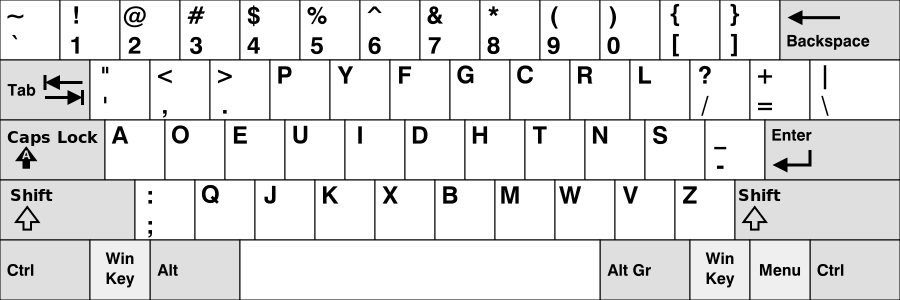
\includegraphics[scale=0.16]{images/KB_United_States_Dvorak.png}
      \caption{\it Dvorak Keyboard}
   \end{minipage}
   \begin{minipage}[b]{0.32\linewidth}   
      \centering 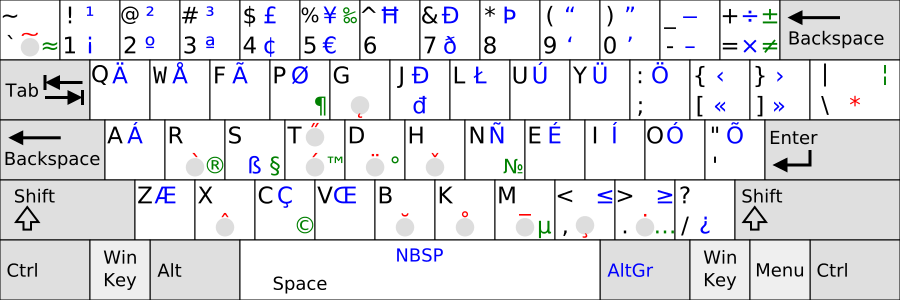
\includegraphics[scale=0.16]{images/KB_US-Colemak_with_AltGr.png}
      \caption{\it Colemak Keyboard}
   \end{minipage}
   \begin{minipage}[b]{0.32\linewidth}
      \centering 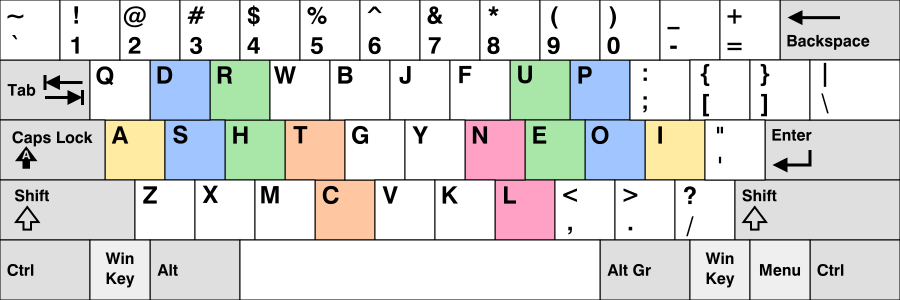
\includegraphics[scale=0.16]{images/KB_English_Workman.png}
      \caption{\it Workman Keyboard}
   \end{minipage}
\end{figure}
\clearpage

\section{Typing way and Fingers position}
To improve typing speed, in addition to change our keyboard, the only way is to practice. Actually, the average typing speed, calculate in Word Per Minute (WPM), is of 44 words.\cite{ref7} In the English language, the fastest typist in the world was Stella Pajunas who had a top speed of 216 words per minute. She realize it on a typewriter in 1946. Nowadays, it is easy with practice to had a typing speed of about 100 words par minute.\\ 
The typing way, which can be learn and improve on a lots of software and websites, is really the most important things to take in consideration to improve our typing speed. This typing way include the position of hands on a keyboard, which will change according to the type of keyboard, but for a QWERTY one it is like the figure 4 shows.
\begin{figure}[H]
\begin{center}
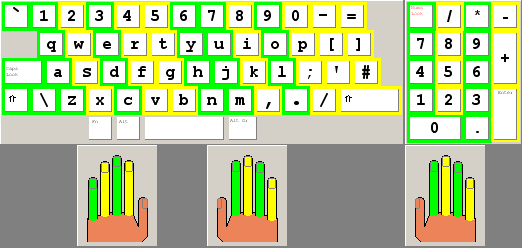
\includegraphics[width=9cm]{images/FingerHandPosUSA.png} 
\end{center}
\caption{\it Fingers position on QWERTY keyboard}
\label{Poulpy est multicolore}
\end{figure}
Here you can find some example of typing test on the internet:
\begin{itemize}
\item\it TypingTest.com\cite{ref8}
\item\it 10fastfingers.com\cite{ref9}
\end{itemize}
It also possible to find typing lessons on the internet.\\
To conclude about this part we can say that way to type and typing speed are things very democratize on the internet especially with a lots of website who can explain you best way to type, position of hands, give you advice and way to improve your typing style with speed test. That is showing that the development of a typing test is something useful.
Every book and website available regarding improving the typing speed are first mentions the finger positions.\\
As the book written by \citet{beginners}, the fingers must be positioned on the \textit{baseline}. The baseline, is the line on the keyboard containing the letters \textit{F} and \textit{J}. As with 'touch typing in ten lessons' \cite{tenlessons} book explains, every fingers should have an assigned letter. The figure below \ref{fing_pos} shows where the finger position is assigned on a QWERTY keyboard.
\begin{figure}[H]
	\centering
	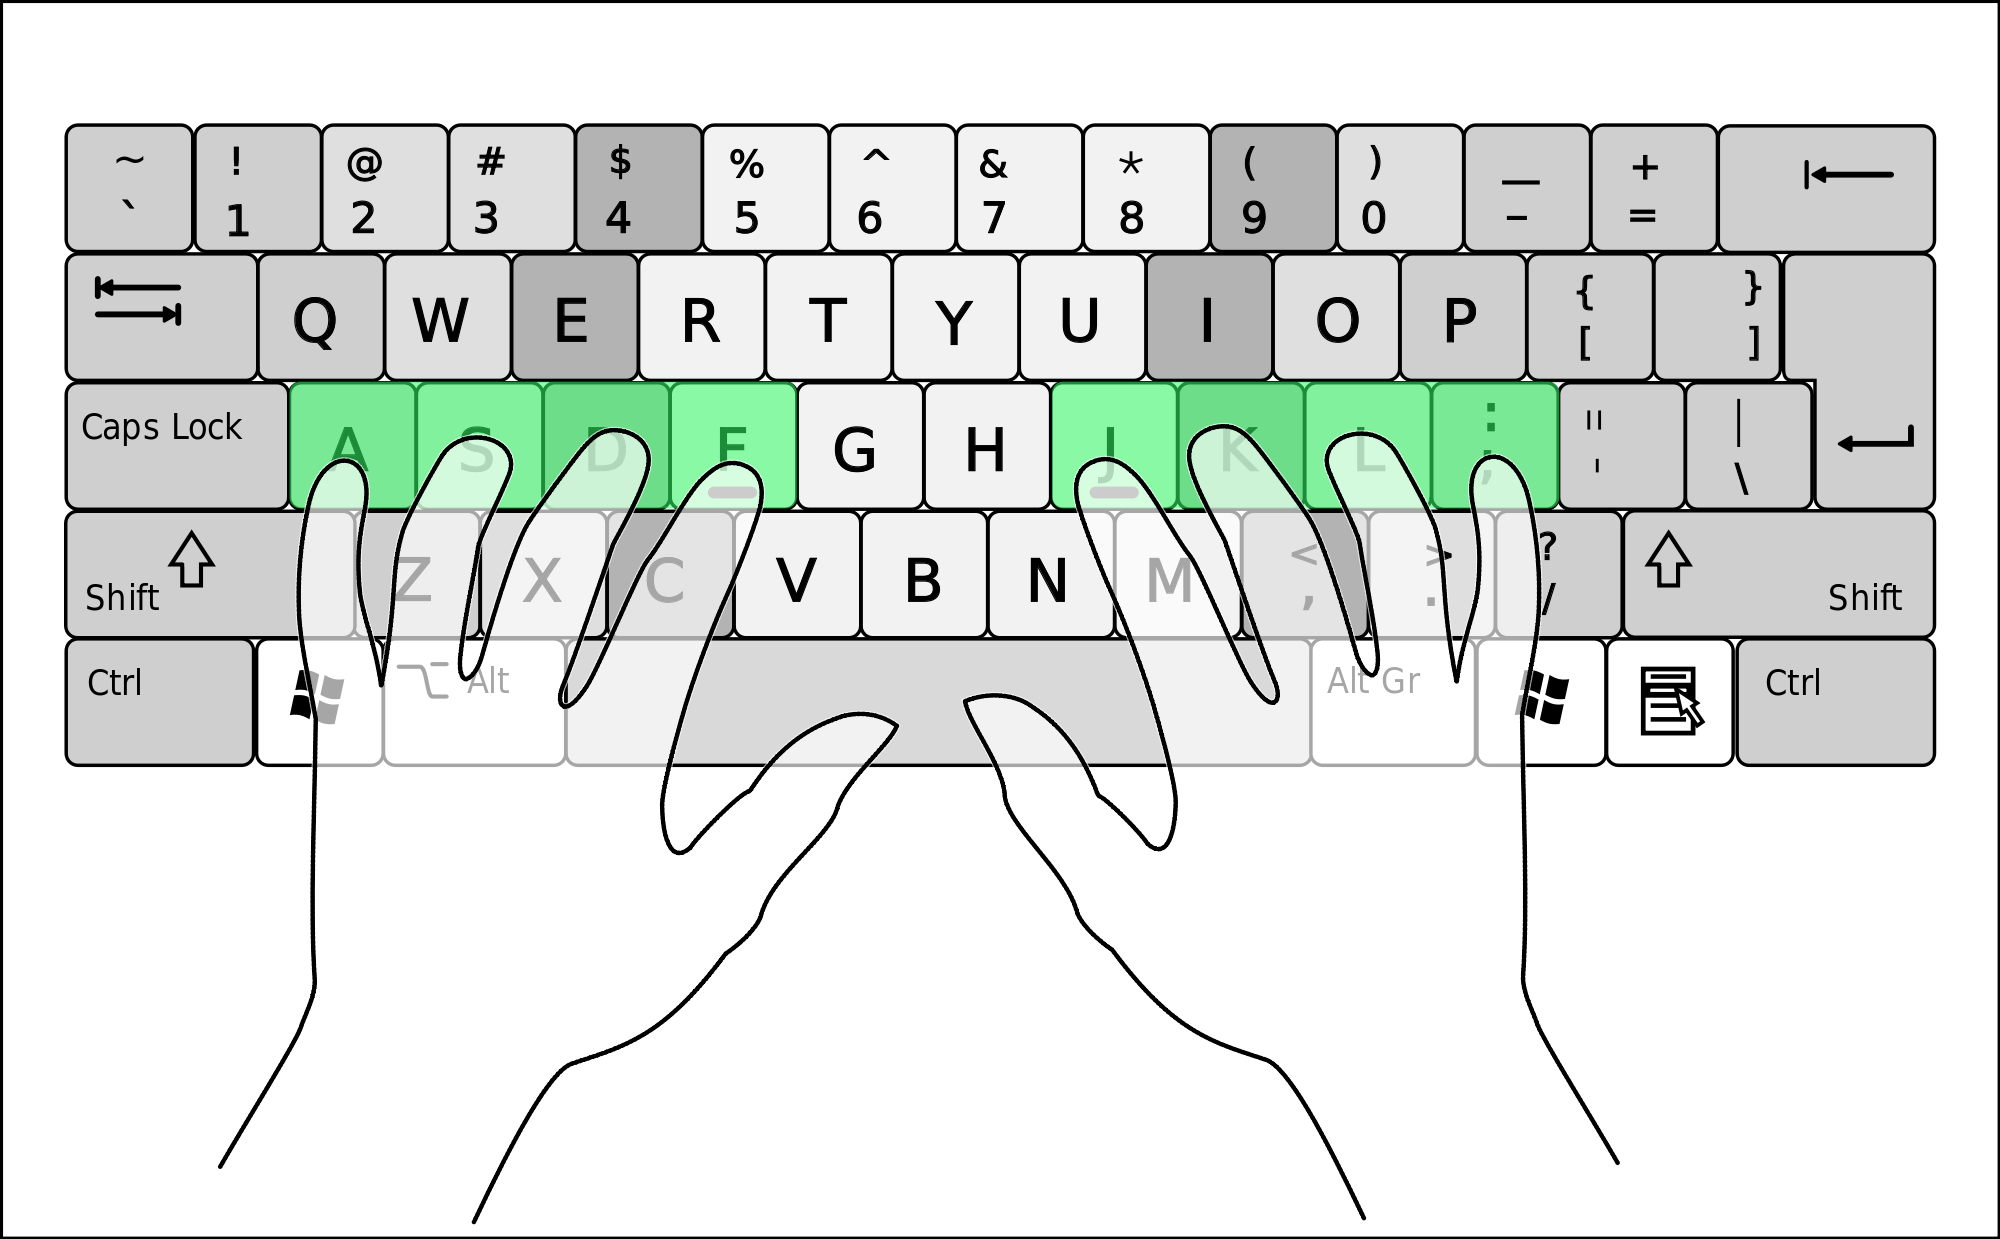
\includegraphics[width=0.7\textwidth]{images/fing_pos.png}
	\caption{Position of the fingers on a QWERTY keyboard}\label{fing_pos}
\end{figure}
However, the layout of the keyboard may vary but the finger position will stay on the same baseline. www.computerhope.com \cite{computerhope} shows the different keys for each finger depending on the keyboard layout.
Other keyboards exist such as those represented in 'typing for beginners' \citep{beginners}. Unfortunately there are not common enough and are only used by more professional typists. So this literature review will not cover the use of them.\\
The user must know which finger is assigned to its specific letter on the keyboard. And so forth for each row. The book written by
\citet{beginners} explains the differents steps on how to follow the assignment for each row. Once again, the letters may vary depending on the keyboard layout, but the finger movements are still the same.
\begin{figure}[H]
    \centering
    \begin{subfigure}[b]{0.3\textwidth}
        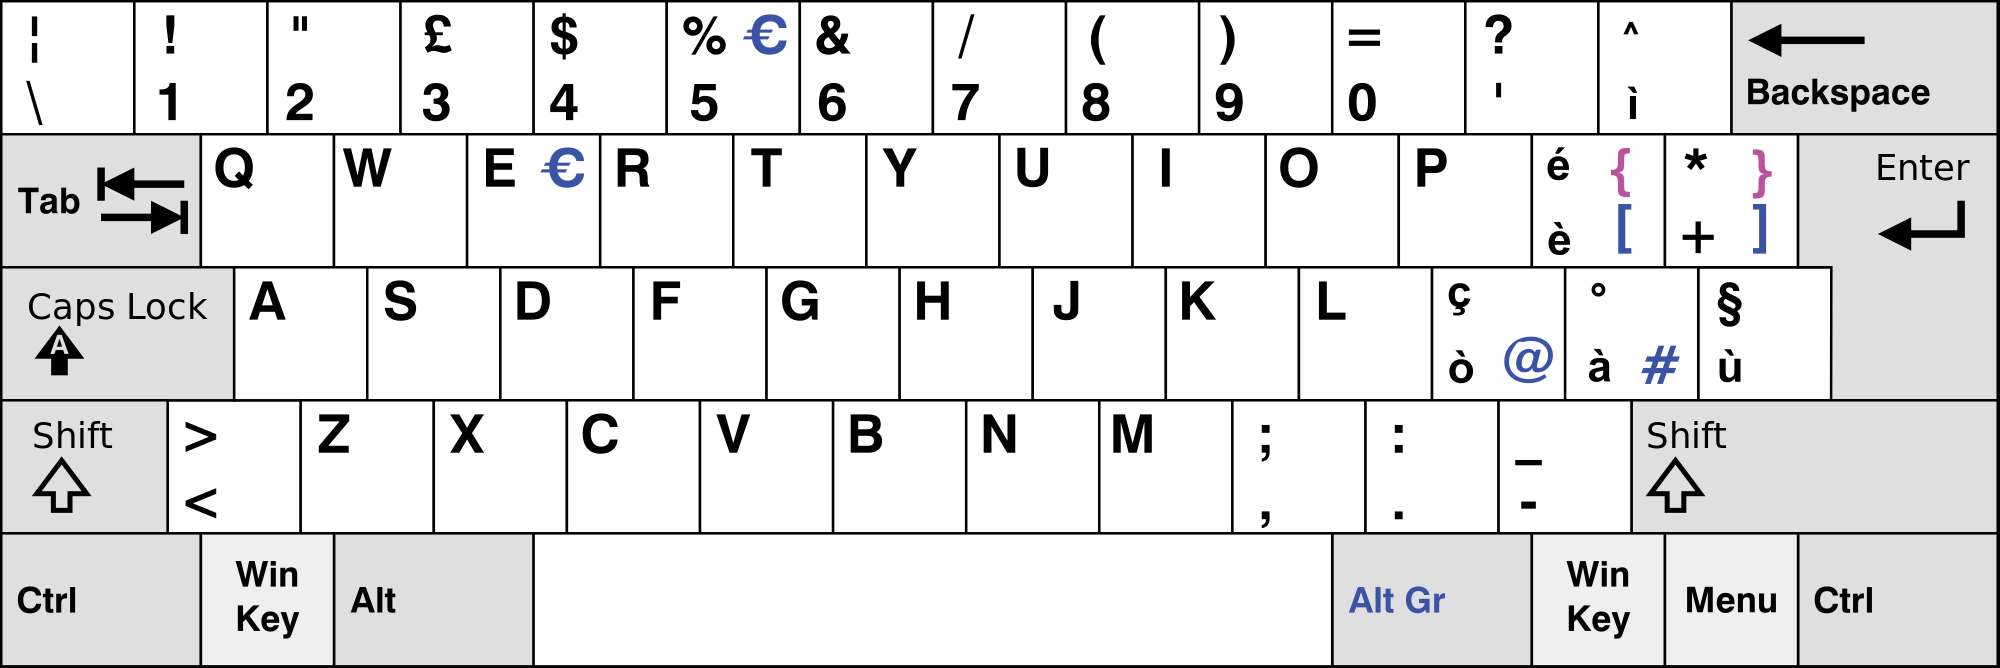
\includegraphics[width=\textwidth]{images/qwerty.png}
        \caption{Qwerty-based layout}
    \end{subfigure}
	 \begin{subfigure}[b]{0.3\textwidth}
        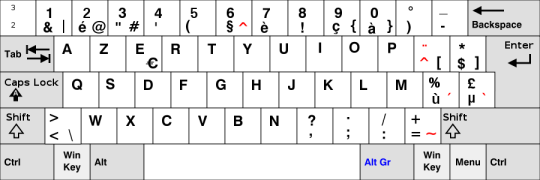
\includegraphics[width=\textwidth]{images/azerty.png}
        \caption{Azerty-based layout}
    \end{subfigure} 
    \begin{subfigure}[b]{0.3\textwidth}
        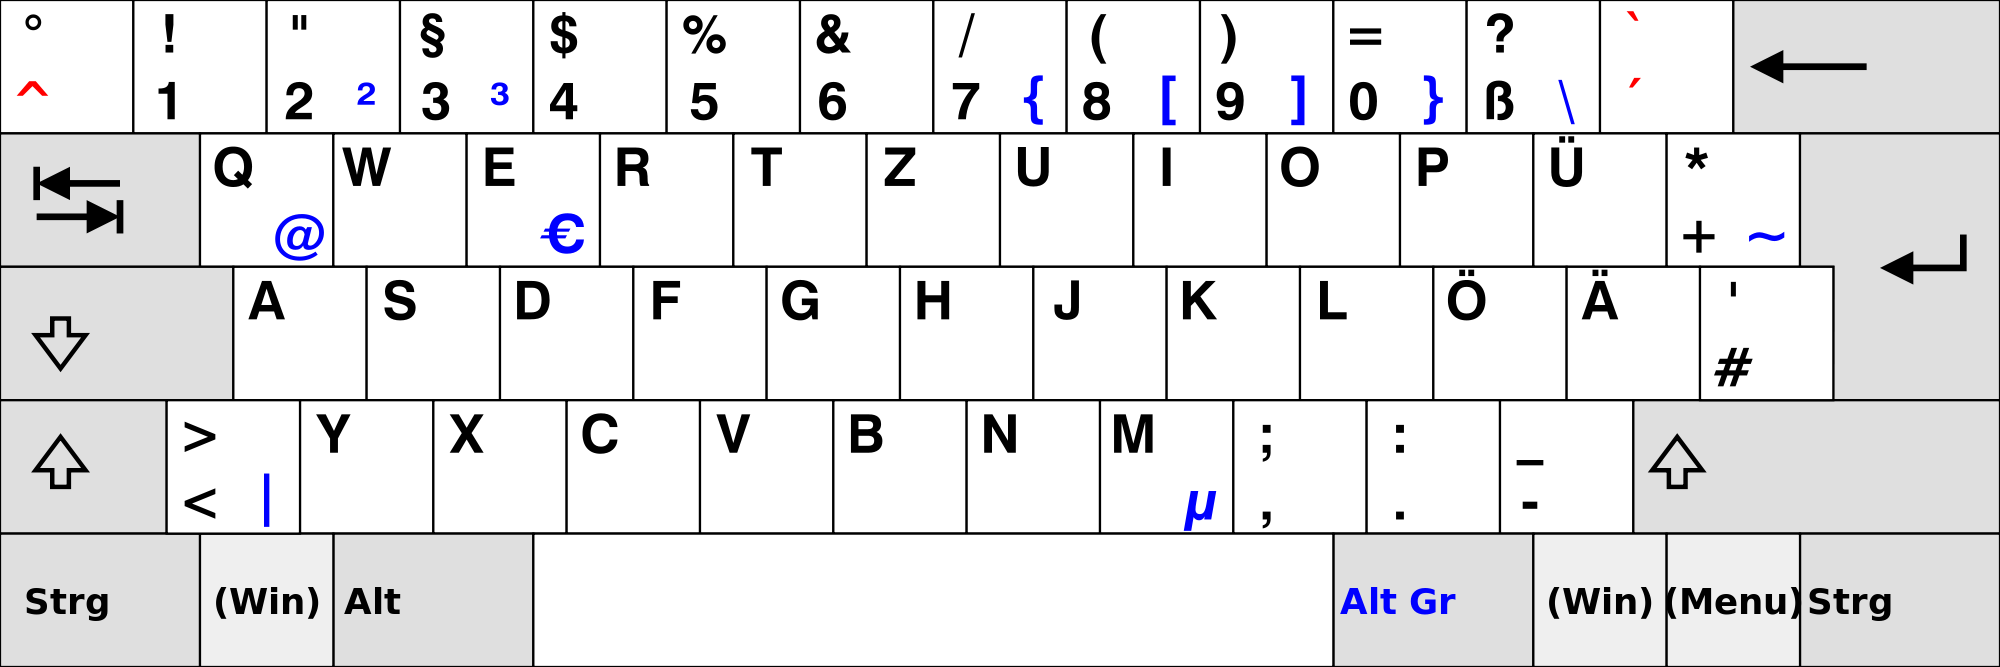
\includegraphics[width=\textwidth]{images/qwertz.png}
        \caption{Qwertz-based layout}
    \end{subfigure}
    \caption{Most common layouts in Europe}
\end{figure}
\clearpage

\section{Practice}
The more you know, the more you type. Once you are able to type a full word one needs to keep practising. This builds up a muscle memory of all the possible key stokes which make up the words of the dictionary.
The computerhope.com\citep{computerhope} website provide good everyday practice example to follow. There is also a large collection of games on the internet to practice and therefore improve the typing speed.\\
how-to-type.com \cite{howto} offers practice sessions such as 10 minutes to an hour per session as their recommendation.
The book written by \citet{handBook} also gives some advice regarding the finger position and the stretch to do beforehand.
There is no software which combines both, doing a check that the user has done finger stretches, and provide advice on how to position yourself in front of the keyboard improving your ability to type correctly. Each of these is done on an individual basis.

\section{Speed and accuracy}
Accuracy is the first skill we need to develop (typing for beginners)\cite{beginners}.\\
Firstly, the user must learn how to type all the letters of the keyboard, as said above. The user must know the exact position of each letter on the keyboard, without having to look at it. Once they know this, they will have the ability to type much faster. However faster can also mean more mistakes. If the mistake is found on the same letter, the user must practice typing this letter again and again to improve accuracy. The problem can also come from a finger which is not reactive enough. In this case, steps need to be put in place in order to train that particular finger. This will be one of the goals of the software to be created. Also, the user must be aware that the more improvement regarding typing speed, the harder it will become to improve this speed.(lingholic.com) \cite{plateau}. Below are two graphs explaining the difference between the expected learning curve and the actual learning curve.

\begin{figure}[H]
    \centering
    \begin{subfigure}[b]{0.4\textwidth}
        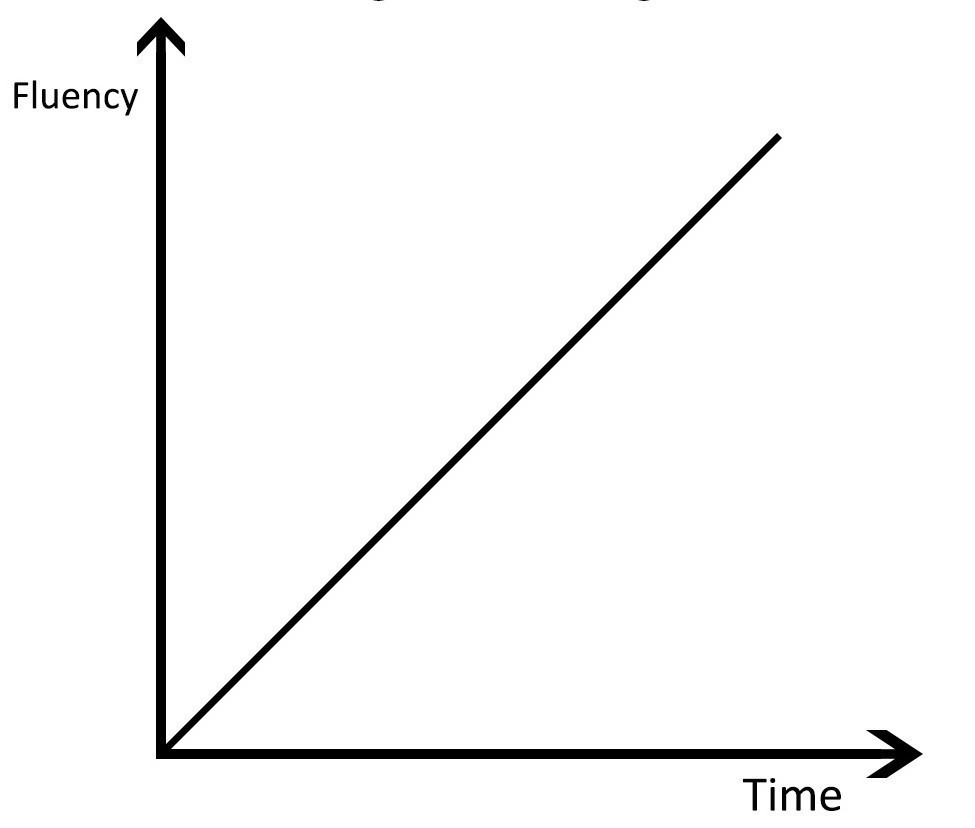
\includegraphics[width=\textwidth]{images/expected.jpg}
        \caption{Expected learning curve}
    \end{subfigure}
    \begin{subfigure}[b]{0.4\textwidth}
        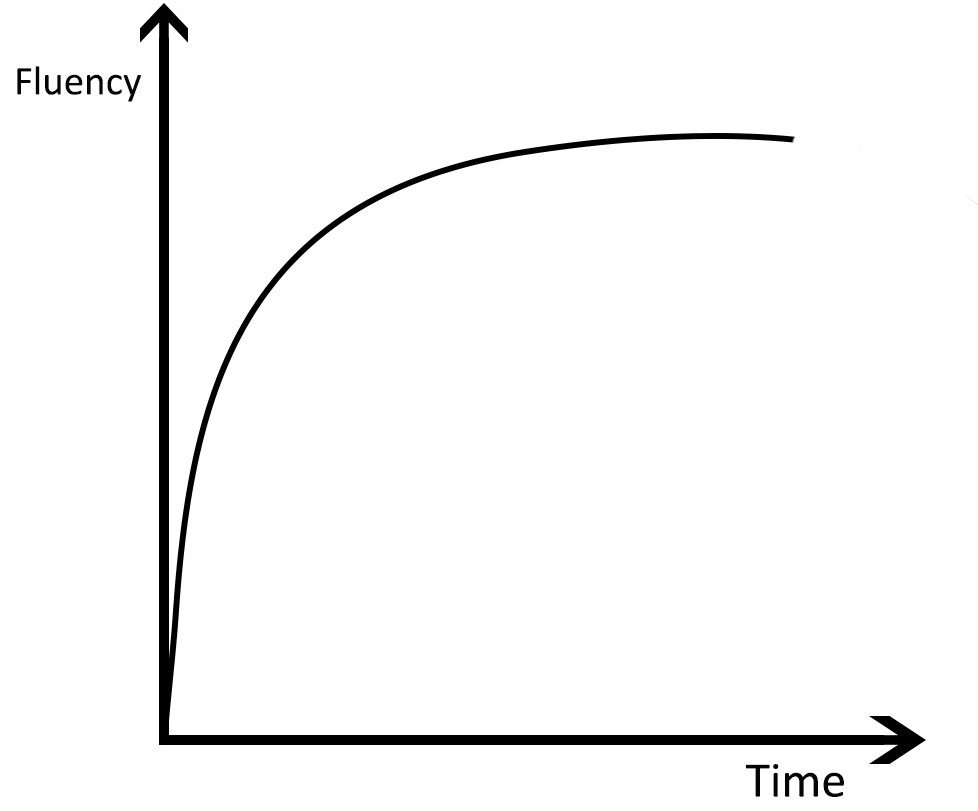
\includegraphics[width=\textwidth]{images/actual.jpg}
        \caption{Actual learning curve}
    \end{subfigure}
    \caption{Expected and actual learning curve}
\end{figure}

\clearpage
\chapter{Conclusion}
From the current knowledge in typing, it appears that it is possible to quickly easily to learn to type faster and with a good accuracy. It is important for the user to learn the basics of the keyboard and the position of the letters. Once this is known, with the time and practice, typing speed will slowly and steadily increase.\\
Whenever the user has some accuracy problem with a single finger, practice will increase general precision.\\
For the general public, it they have a computer and a keyboard, they can learn how to type faster in three steps :
\begin{itemize}
	\item Learn the position of the letters on the keyboard and associate each fingers to each key
	\item Practice in order to improve the speed
	\item Correct the accuracy problems
\end{itemize}

\clearpage

%Bibliography
\begin{flushleft}
	\bibliographystyle{unsrtnat}
	\bibliography{lit_review.bib}
\end{flushleft}

\clearpage
\afterpage{\blankpage}

\end{document}
\chapter*{Keywords}
\begin{sortedlist}
  \sortitem{Keyboard}
  \sortitem{Keyboard layout}
  \sortitem{Fingers}
  \sortitem{Keys}
  \sortitem{Speed}
  \sortitem{Accuracy}
  \sortitem{Typing}
  \sortitem{Improvements}
  \sortitem{Learning}
\end{sortedlist}

\thispagestyle{empty}
\clearpage

\setcounter{page}{1}
\chapter{Abstract}
This review explores the way of improving the typing speed on the common keyboard.
Today's world is already full of keyboards, and it will never cease to increase. To be more efficient when using a computer, it is a good idea to learn how to type. On the web there are plenty of sources to improve your skills, but there is very little of them who really teach you how to type faster from scratch. The same goes for the existing software. And the main issue regarding this is that the software is not free.\\
The work presented here is based on books and websites that give advice on how to type speedily.\\
In order to address that issue, this review looks at the finger positions. Then it goes on to discuss how the user must practice to improve his or her typing skills. Lastly, it looks at the importance of accuracy and how this outweighs speed.

\clearpage
\chapter{Literature review}
\section{Some history}
In 1890, Lovisa Ellen Barnes wrote a book called "How To Become Expert in Typewriting"\cite{ref2} who was explaining how type on a Remington Typewriter.\\
In 1915, Dr. Henry Faulds wrote a book called "A Manual of Practical Dactylography"\cite{ref3}\\
An other example of book talking about dactylography.\cite{ref5}\\   
A more recent one published in 2012 and wrote by Faulds H.\cite{ref4}\\
As we can see, from a long time people provide way to learn how type so we can thereby say that way to type, and so typing speed, are always being important and are never been neglect by people.\\

\section{Keyboard}
The original layouts for the first mechanical typewriters were in alphabetical order (ABCDE etc..). Then different type of keyboard appeared according to languages used in each country (the most used is the QWERTY one but you can find AZERTY in France or QWERTZ in Germany for example).\\
Each of this layouts keyboard are classics one, that is mean when you buy a keyboard you will have one of this, but, since the invention of computers and indeed keyboards, a lots of research 	conducted to the invention of new non-classics layouts. Indeed, this new layouts had to made typing more easy and more comfortable. The most famous are Dvorak, Colemak and Workman.\\
Dvorak has been invented by August Dvorak and is the best alternative to QWERTY. It has been designed to increase typing speed, decrease errors and increase comfort.\\
After Dvorak, Colemak is the most popular. Also based on the QWERTY keyboard, it has been created in 2006 by Shai Coleman. It allow to promote the bearing of fingers on the middle rows of keys, it is better to maximise alternation between use right and left hands and minimize the movement of hands on the keyboard.\\
The third one is Workman. Thise one is less used than Dvorak and Colemak, but according with different developers, it is actually the best one to reduce fingers exhaustion. Indeed, it reduce usage of the two middle columns, reduce horizontal,diagonal and vertical finger stretching compared to Dvorak and Colemak.\cite{ref6}\\
To conclude about that, we can obviously say that from people have always trying to increase their typing skills by inventing new keyboards layouts which increase typing comfort and thus typing speed.     
\begin{figure}[h!]
   \begin{minipage}[b]{0.32\linewidth}
      \centering 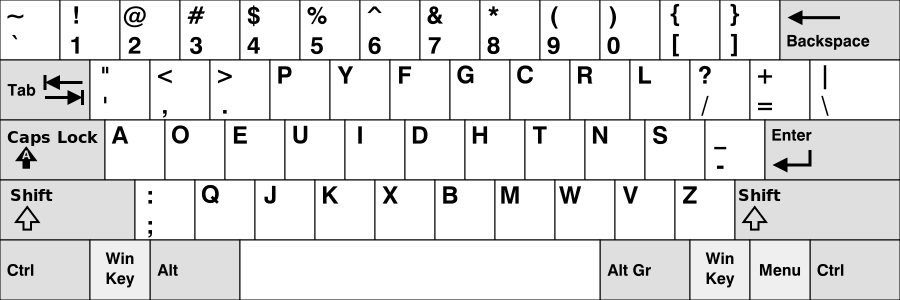
\includegraphics[scale=0.16]{images/KB_United_States_Dvorak.png}
      \caption{\it Dvorak Keyboard}
   \end{minipage}
   \begin{minipage}[b]{0.32\linewidth}   
      \centering 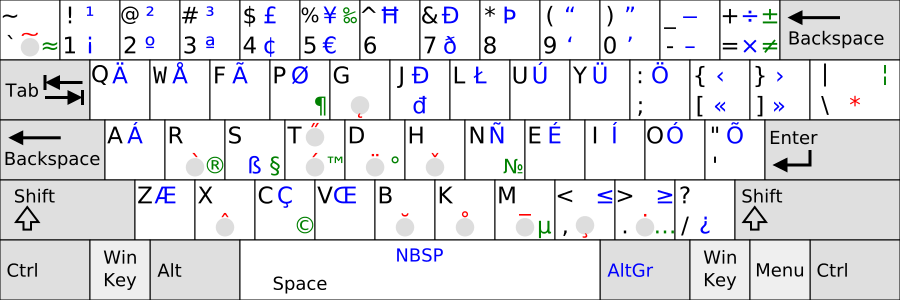
\includegraphics[scale=0.16]{images/KB_US-Colemak_with_AltGr.png}
      \caption{\it Colemak Keyboard}
   \end{minipage}
   \begin{minipage}[b]{0.32\linewidth}
      \centering 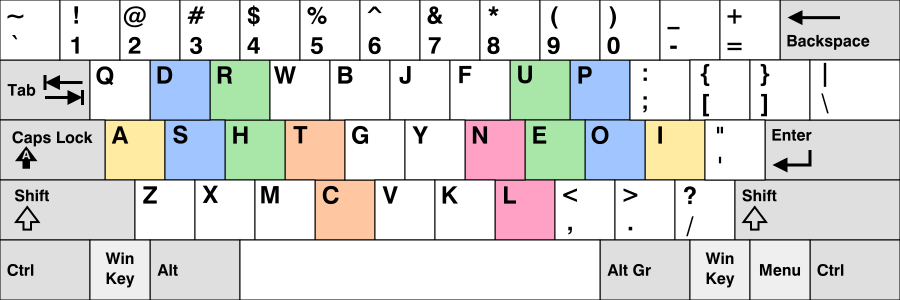
\includegraphics[scale=0.16]{images/KB_English_Workman.png}
      \caption{\it Workman Keyboard}
   \end{minipage}
\end{figure}
\clearpage

\section{Typing way and Fingers position}
To improve typing speed, in addition to change our keyboard, the only way is to practice. Actually, the average typing speed, calculate in Word Per Minute (WPM), is of 44 words.\cite{ref7} In the English language, the fastest typist in the world was Stella Pajunas who had a top speed of 216 words per minute. She realize it on a typewriter in 1946. Nowadays, it is easy with practice to had a typing speed of about 100 words par minute.\\ 
The typing way, which can be learn and improve on a lots of software and websites, is really the most important things to take in consideration to improve our typing speed. This typing way include the position of hands on a keyboard, which will change according to the type of keyboard, but for a QWERTY one it is like the figure 4 shows.
\begin{figure}[H]
\begin{center}
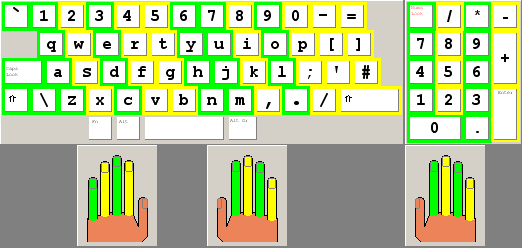
\includegraphics[width=9cm]{images/FingerHandPosUSA.png} 
\end{center}
\caption{\it Fingers position on QWERTY keyboard}
\label{Poulpy est multicolore}
\end{figure}
Here you can find some example of typing test on the internet:
\begin{itemize}
\item\it TypingTest.com\cite{ref8}
\item\it 10fastfingers.com\cite{ref9}
\end{itemize}
It also possible to find typing lessons on the internet.\\
To conclude about this part we can say that way to type and typing speed are things very democratize on the internet especially with a lots of website who can explain you best way to type, position of hands, give you advice and way to improve your typing style with speed test. That is showing that the development of a typing test is something useful.
Every book and website available regarding improving the typing speed are first mentions the finger positions.\\
As the book written by \cite{beginners}, the fingers must be positioned on the \textit{baseline}. The baseline, is the line on the keyboard containing the letters \textit{F} and \textit{J}. As with 'touch typing in ten lessons' \cite{tenlessons} book explains, every fingers should have an assigned letter. The figure below \ref{fing_pos} shows where the finger position is assigned on a QWERTY keyboard.
\begin{figure}[H]
	\centering
	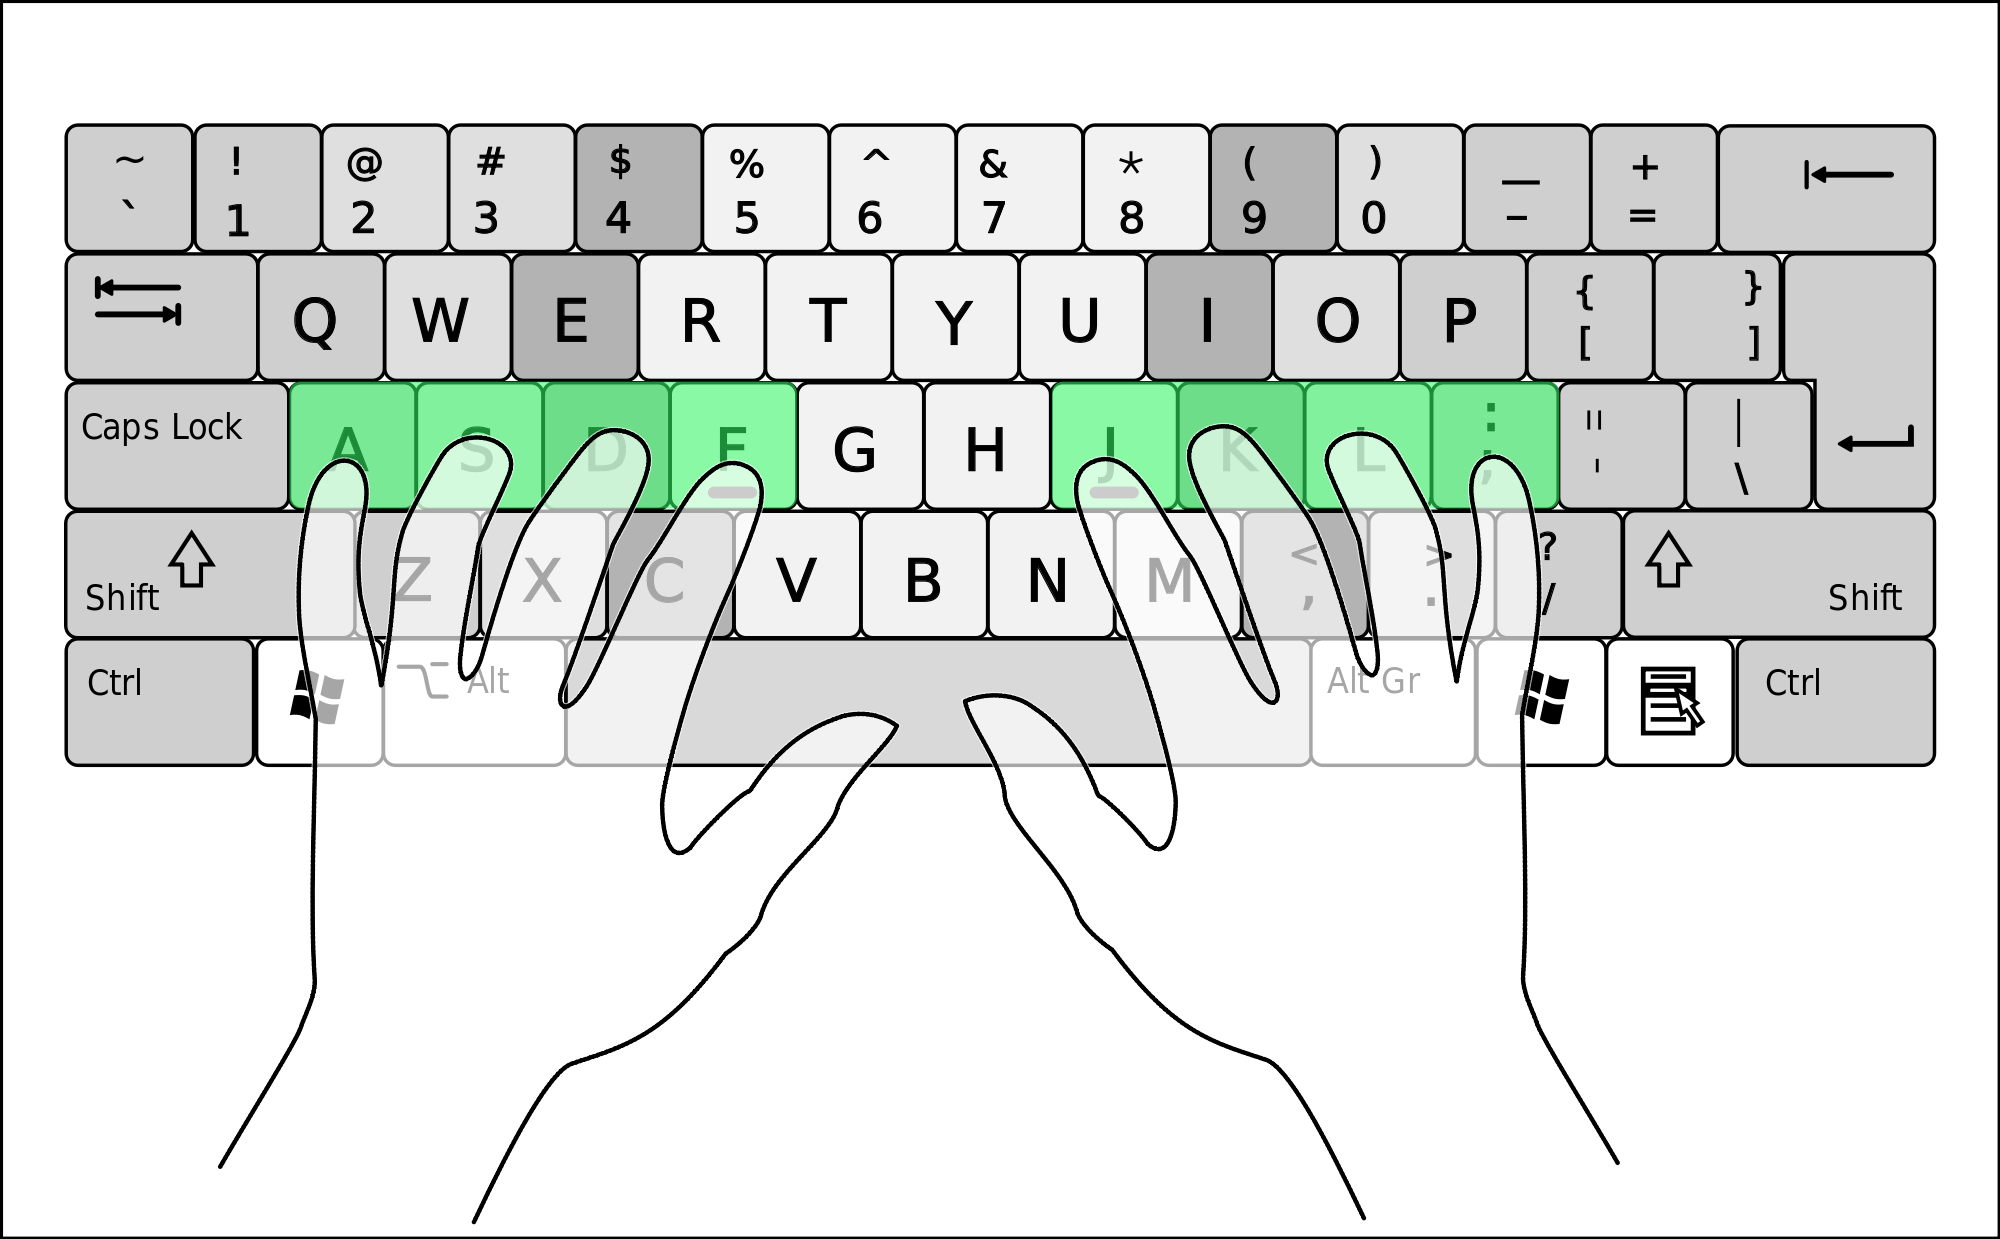
\includegraphics[width=0.7\textwidth]{images/fing_pos.png}
	\caption{Position of the fingers on a QWERTY keyboard}\label{fing_pos}
\end{figure}
However, the layout of the keyboard may vary but the finger position will stay on the same baseline. www.computerhope.com \cite{computerhope} shows the different keys for each finger depending on the keyboard layout.
Other keyboards exist such as those represented in 'typing for beginners' \cite{beginners}. Unfortunately there are not common enough and are only used by more professional typists. So this literature review will not cover the use of them.\\
The user must know which finger is assigned to its specific letter on the keyboard. And so forth for each row. The book written by
\cite{beginners} explains the differents steps on how to follow the assignment for each row. Once again, the letters may vary depending on the keyboard layout, but the finger movements are still the same.
\begin{figure}[H]
    \centering
    \begin{subfigure}[b]{0.3\textwidth}
        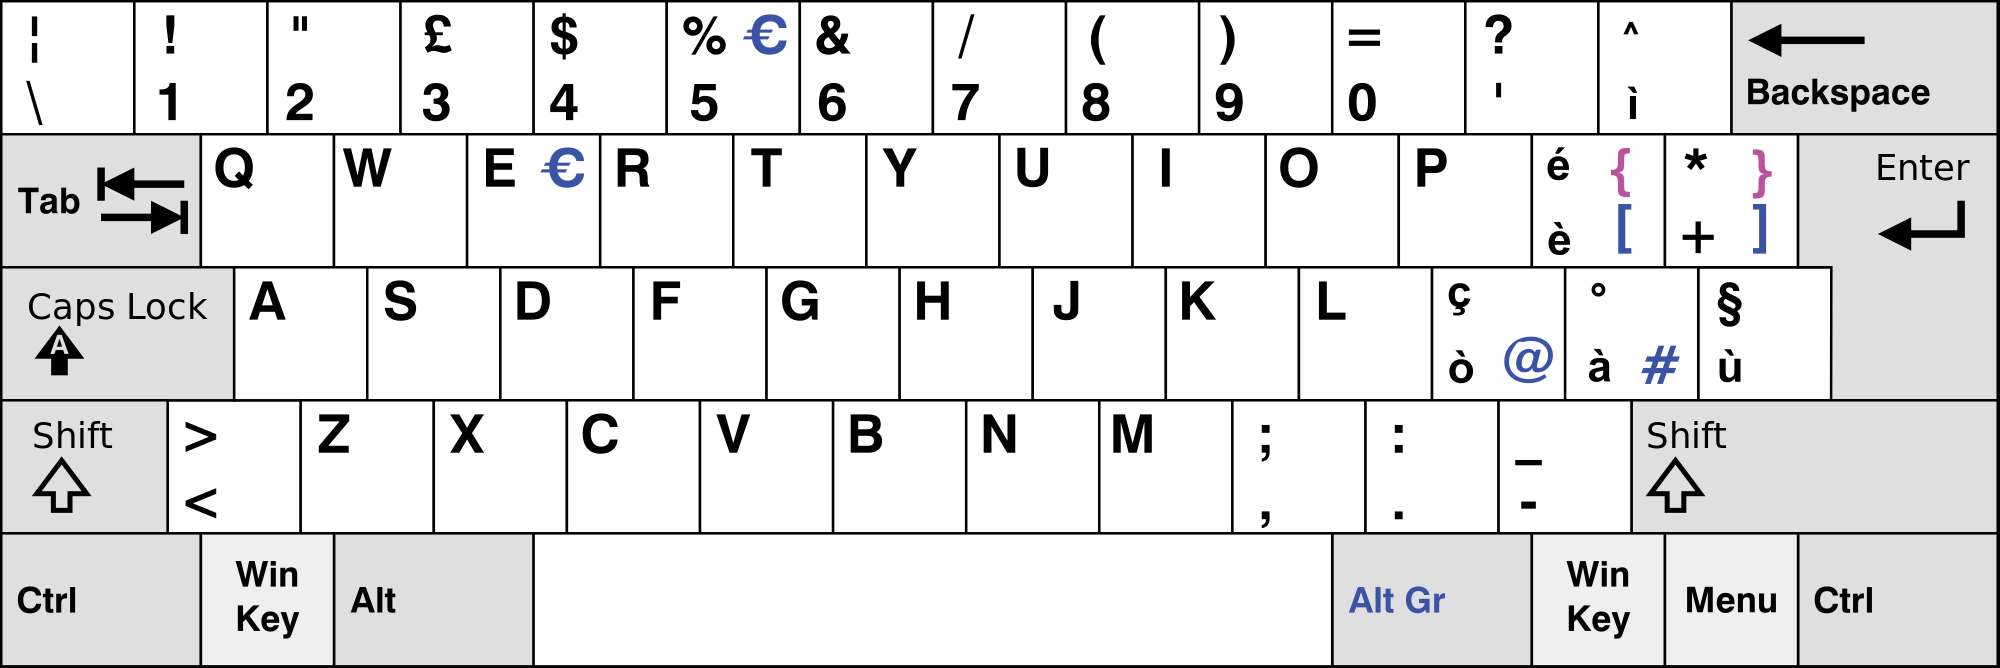
\includegraphics[width=\textwidth]{images/qwerty.png}
        \caption{Qwerty-based layout}
    \end{subfigure}
	 \begin{subfigure}[b]{0.3\textwidth}
        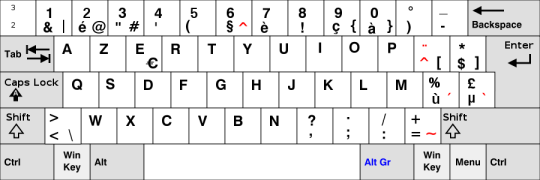
\includegraphics[width=\textwidth]{images/azerty.png}
        \caption{Azerty-based layout}
    \end{subfigure} 
    \begin{subfigure}[b]{0.3\textwidth}
        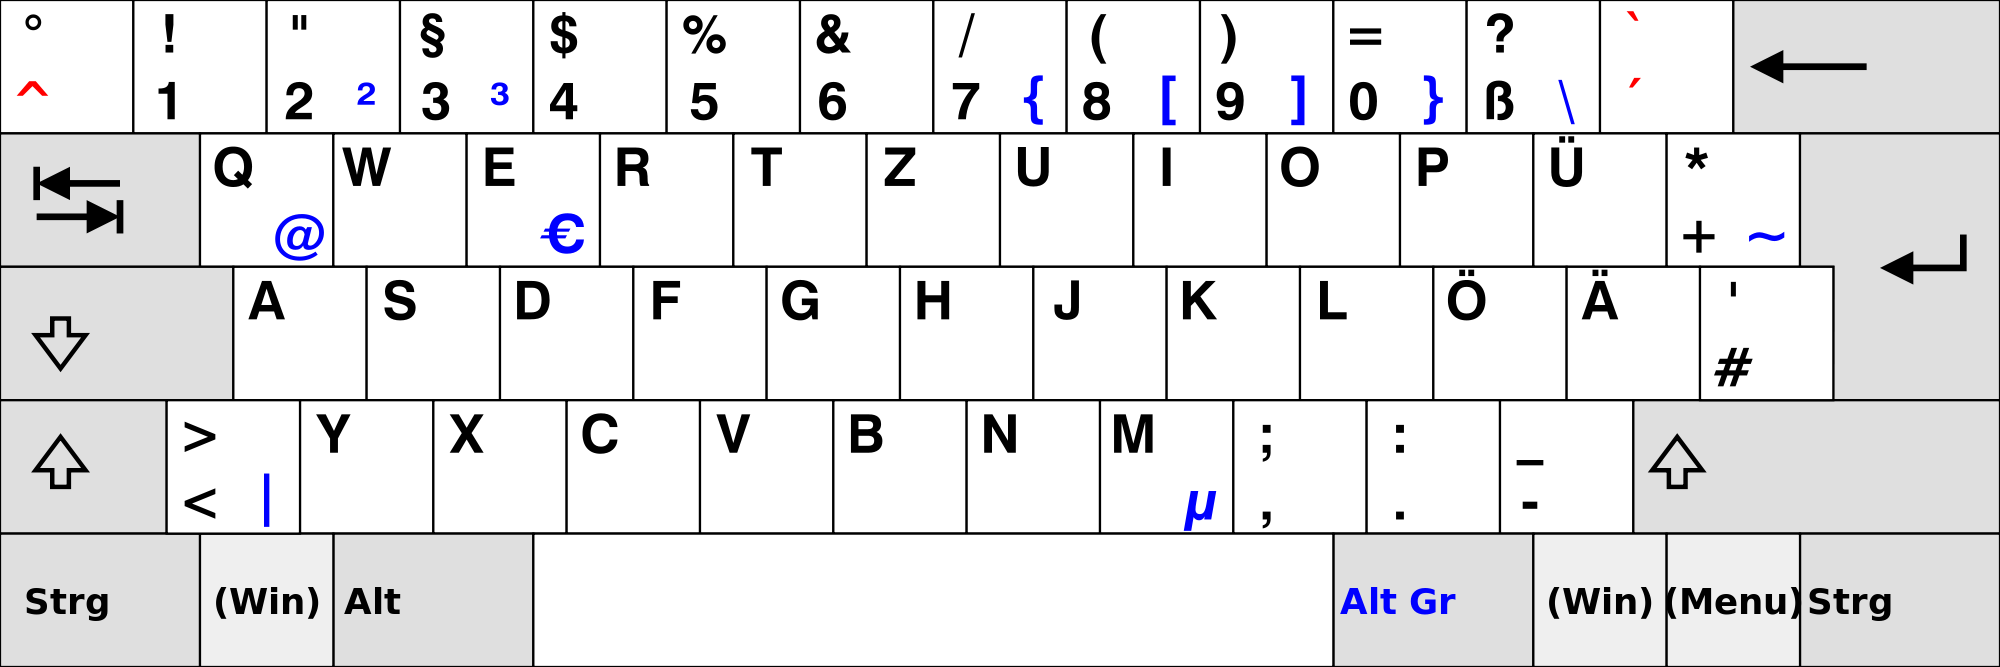
\includegraphics[width=\textwidth]{images/qwertz.png}
        \caption{Qwertz-based layout}
    \end{subfigure}
    \caption{Most common layouts in Europe}
\end{figure}
\clearpage

\section{Practice}
The more you know, the more you type. Once you are able to type a full word one needs to keep practising. This builds up a muscle memory of all the possible key stokes which make up the words of the dictionary.
The computerhope.com\cite{computerhope} website provide good everyday practice example to follow. There is also a large collection of games on the internet to practice and therefore improve the typing speed.\\
how-to-type.com \cite{howto} offers practice sessions such as 10 minutes to an hour per session as their recommendation.
The book written by \cite{handBook} also gives some advice regarding the finger position and the stretch to do beforehand.
There is no software which combines both, doing a check that the user has done finger stretches, and provide advice on how to position yourself in front of the keyboard improving your ability to type correctly. Each of these is done on an individual basis.

\section{Speed and accuracy}
Accuracy is the first skill we need to develop (typing for beginners)\cite{beginners}.\\
Firstly, the user must learn how to type all the letters of the keyboard, as said above. The user must know the exact position of each letter on the keyboard, without having to look at it. Once they know this, they will have the ability to type much faster. However faster can also mean more mistakes. If the mistake is found on the same letter, the user must practice typing this letter again and again to improve accuracy. The problem can also come from a finger which is not reactive enough. In this case, steps need to be put in place in order to train that particular finger. This will be one of the goals of the software to be created. Also, the user must be aware that the more improvement regarding typing speed, the harder it will become to improve this speed.(lingholic.com) \cite{plateau}. Below are two graphs explaining the difference between the expected learning curve and the actual learning curve.

\begin{figure}[H]
    \centering
    \begin{subfigure}[b]{0.4\textwidth}
        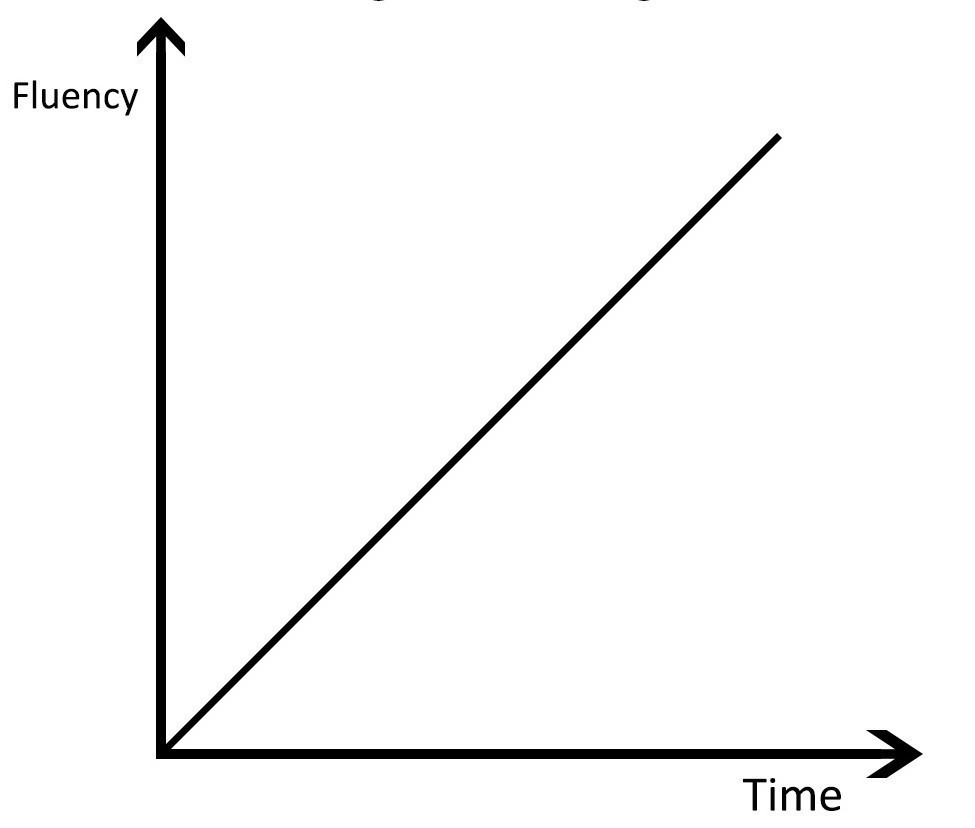
\includegraphics[width=\textwidth]{images/expected.jpg}
        \caption{Expected learning curve}
    \end{subfigure}
    \begin{subfigure}[b]{0.4\textwidth}
        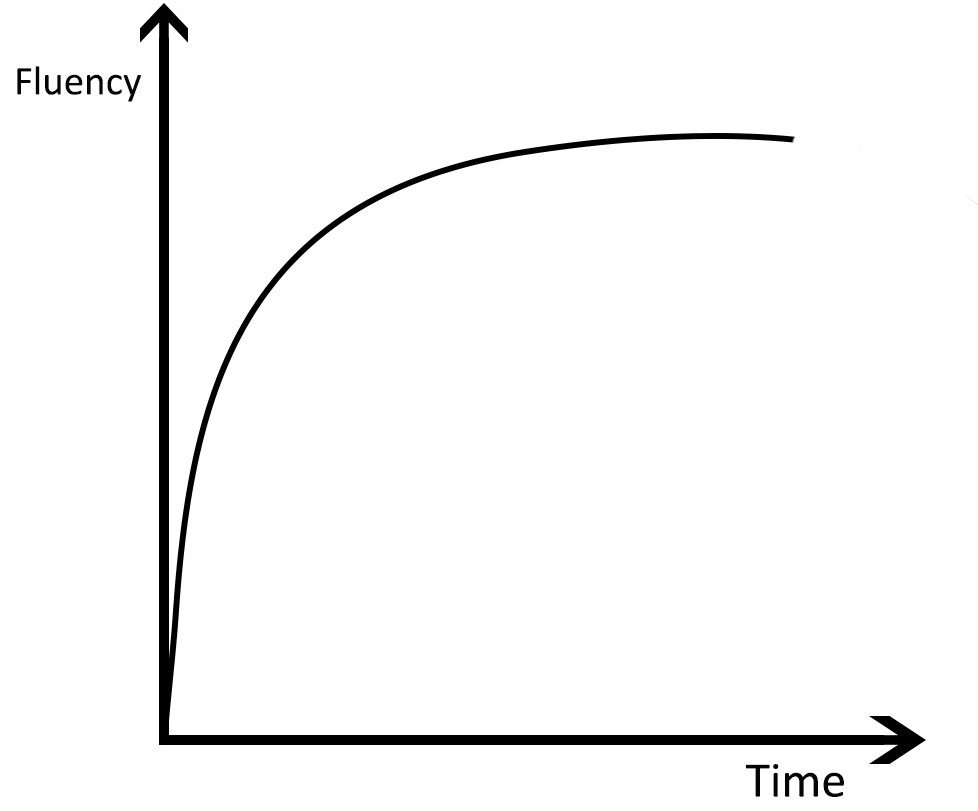
\includegraphics[width=\textwidth]{images/actual.jpg}
        \caption{Actual learning curve}
    \end{subfigure}
    \caption{Expected and actual learning curve}
\end{figure}

\clearpage
\chapter{Conclusion}
From the current knowledge in typing, it appears that it is possible to quickly easily to learn to type faster and with a good accuracy. It is important for the user to learn the basics of the keyboard and the position of the letters. Once this is known, with the time and practice, typing speed will slowly and steadily increase.\\
Whenever the user has some accuracy problem with a single finger, practice will increase general precision.\\
For the general public, it they have a computer and a keyboard, they can learn how to type faster in three steps :
\begin{itemize}
	\item Learn the position of the letters on the keyboard and associate each fingers to each key
	\item Practice in order to improve the speed
	\item Correct the accuracy problems
\end{itemize}

\clearpage

%Bibliography
\begin{flushleft}
	\bibliographystyle{plain}
	\bibliography{lit_review}
\end{flushleft}

\part{System analysis}

\chapter{Functional requirements}
As C++ need to be compile, we can provide to users an executable which is the only thing they need to run the software on their computer.

\section{What the software does}
This application is a learning and testing software using Qt framework and develop with C++ language. The software provide a way for users to learn from the beginning how type fast and well on a keyboard.
\\
The learning part is divided in forty-eight sections ("Learn" part in the GUI), each one gives to the user a training for different couple of letter. At the beginning when the user account is new, only the first training is available. When a user select a training couple, a keyboard layout is display (related to the layout the user select in his parameters) explaining where the letters are on the keyboard and which finger use for both. The first couple is "fj". When the training for the couple is completed, the training for the next couple is unlocked. The second couple is "dk", so when the user will start this training, he will start to type on 'd' or 'k' letter on the keyboard. However as the user type, letters from the first training will appears and user will now have to type on 'd','k','f' or 'j'. This process is the same for all along of the forty-eight learning sections, each time the user will have to manage the new couple of letter as well as the old ones.
\\
The practice part is divided in four sections ("Practice" part in the GUI), each one gives to the user an exercise. The first type of exercise is "Against time". As his name say, users has to type most words as possible in two minutes. At the end the software display some information, especially the number of word per minute.\\
The second type of exercise is "Normal", the software display a list of word, only in small letter, and the user has to type faster as possible and as before the application displays informations at the end.\\
The third type of exercise is "Improve". This one is a bit similar to learning exercise. Indeed it is based on the principal of repetition of some couple of letter that you have to type faster as possible.\\
The last type of exercise is "Text". This one is the most complete exercise because it regroups all you have learned before. Indeed, the text display contains small and capital letters, punctuation and word some words can be complex.
\\
The statistics part ("Statistics" part in the GUI) provides a way for users to get some statistics and is a good way for the user to get a rapid overview of his progression.
\\
The game part ("Game" part in the GUI) provides an interactive keyboard where user can see with which finger each letter on the keyboard may be type.
          

\section{Systems and subsystems}
The application contain one main system which is the software itself. As C++ is a language which need to be compile, the compilation provide a executable which is the only thing users need to run the software.
We do not need database to store any data, everything is stored in different files using DataStream.  

\section{Data requirements}
As said before, data are stored in different files using DataStream or a Qt class called QSettings. DataStrems is well support by Qt and is used to store informations in files. It is possible then to also read those files. QSettings is a class provide in the Qt library and can be used to store informations directly on the user desktop.

\subsection{Diagrams}
Next figures respectively shows the relationship diagram (figure \ref{Rhomepage}), the sequence diagram (figure \ref{Shomepage}) and the Use Case diagram (figure \ref{UChomepage}) (without details) for the home page. Basically, the home page works like this:
\begin{itemize}
\item The user start the software which is going to start the system and displaying the home page.
\item The user will have the choice between select and delete an existing user or create a new one. Those action are going to call different functions.
\end{itemize}

\begin{figure}[H]
	\centering
	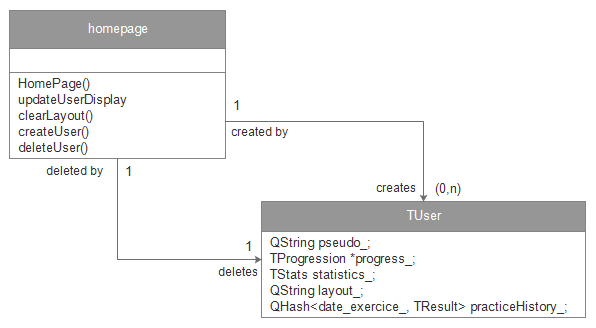
\includegraphics[width=12cm]{diagrams/Rhomepage.png}
	\caption{Relationship diagram for Home page}
	\label{Rhomepage} 
\end{figure}
\begin{figure}[H]
	\centering
	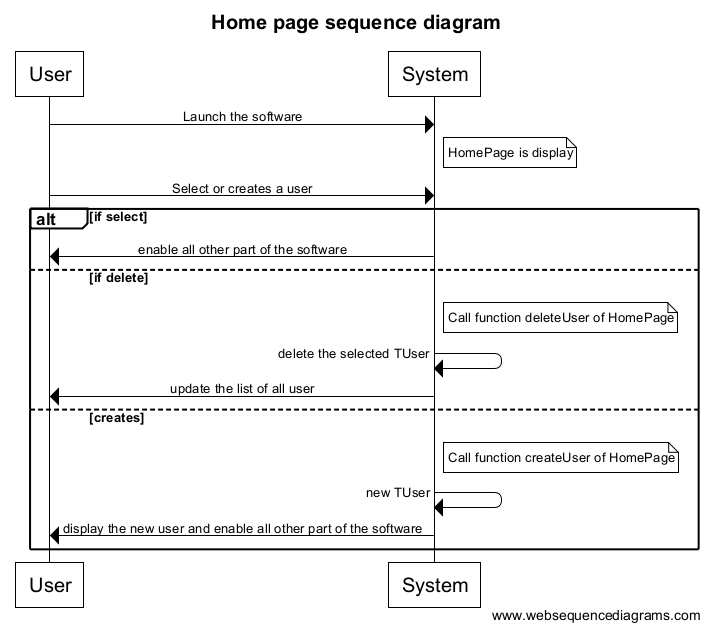
\includegraphics[width=12cm]{diagrams/Shomepage.png}
	\caption{Sequence diagram for Home page}
	\label{Shomepage}
\end{figure}
\begin{figure}[H]
	\centering
	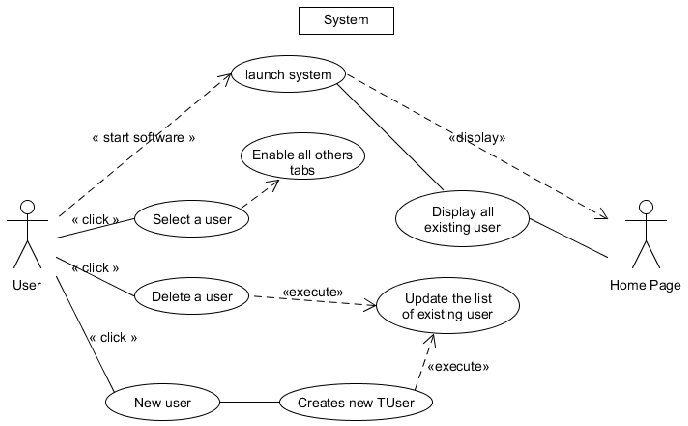
\includegraphics[width=12cm]{diagrams/UChomepage.png}
	\caption{User case diagram for Home page}
	\label{UChomepage}
\end{figure}

Next figures respectively shows the relationship diagram (figure \ref{Rlearnpage}), the sequence diagram (figure \ref{Slearnpage}) and the Use Case diagram (figure \ref{UClearnpage}) (without details) for the learn page. Basically, the learn page works like this:
\begin{itemize}
\item The user has already start the software and selected a user.
\item The system shows all learning exercise to the user (including already done and no done yet exercise).
\item The user the exercise he want and the system display the corresponding one in a new window.
\item When the exercise is done the system shows the results to the user.
\end{itemize}

\begin{figure}[H]
	\centering
	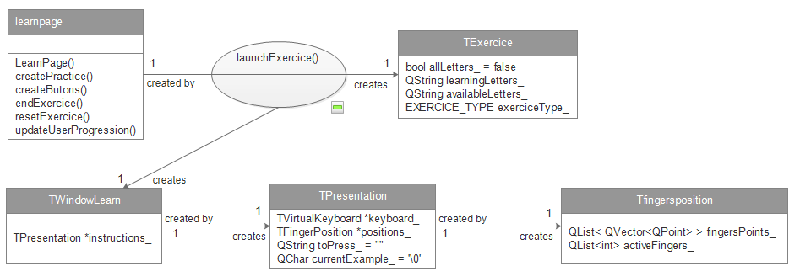
\includegraphics[width=12cm]{diagrams/Rlearnpage.png}
	\caption{Relationship diagram for Learn page}	
	\label{Rlearnpage}
\end{figure}
\begin{figure}[H]
	\centering
	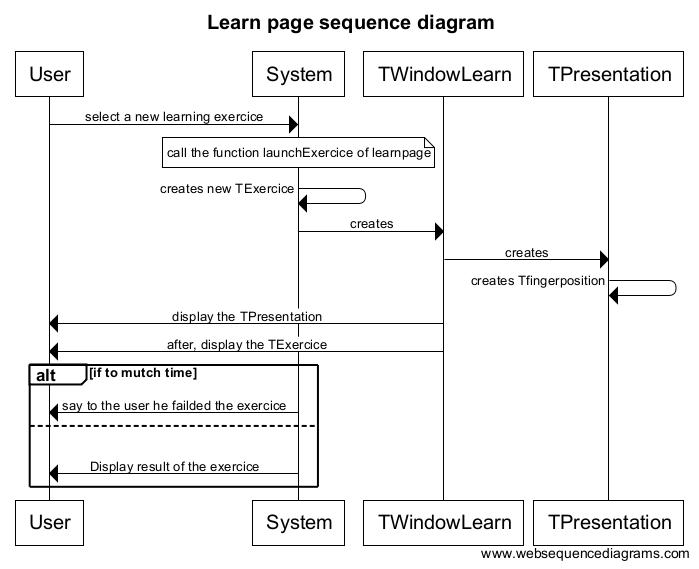
\includegraphics[width=12cm]{diagrams/Slearnpage.png}
	\caption{Sequence diagram for Learn page}
	\label{Slearnpage}
\end{figure}
\begin{figure}[H]
	\centering
	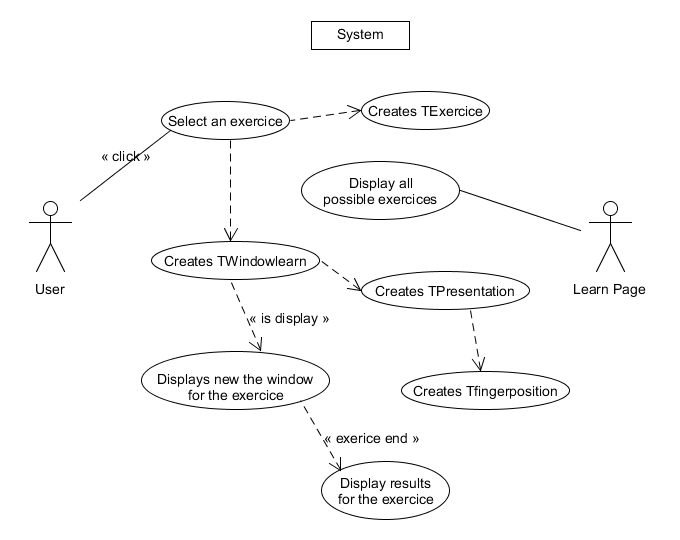
\includegraphics[width=12cm]{diagrams/UClearnpage.png}
	\caption{User case diagram for Leran page}
	\label{UClearnpage}
\end{figure}

Next figures respectively shows the relationship diagram (figure\ref{Rpracticepage}), the sequence diagram (figure\ref{Spracticepage}) and the Use Case diagram (without details) for the practice page. Basically, the practice page works like this:
\begin{itemize}
\item The user has already start the software and selected a user.
\item The system shows all the four different exercise to the user.
\item The user select the one he want and the system will display it in a new window.
\item When the exercise is done the system shows the results to the user.
\end{itemize}

\begin{figure}[H]
	\centering
    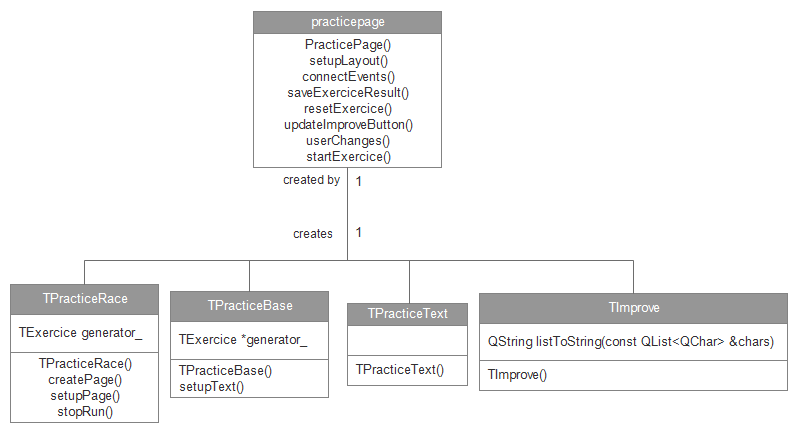
\includegraphics[width=12cm]{diagrams/Rpracticepage.png}
    \caption{Relationship diagram for Practice page}  
    \label{Rpracticepage} 
\end{figure}
\begin{figure}[H]
	\centering
    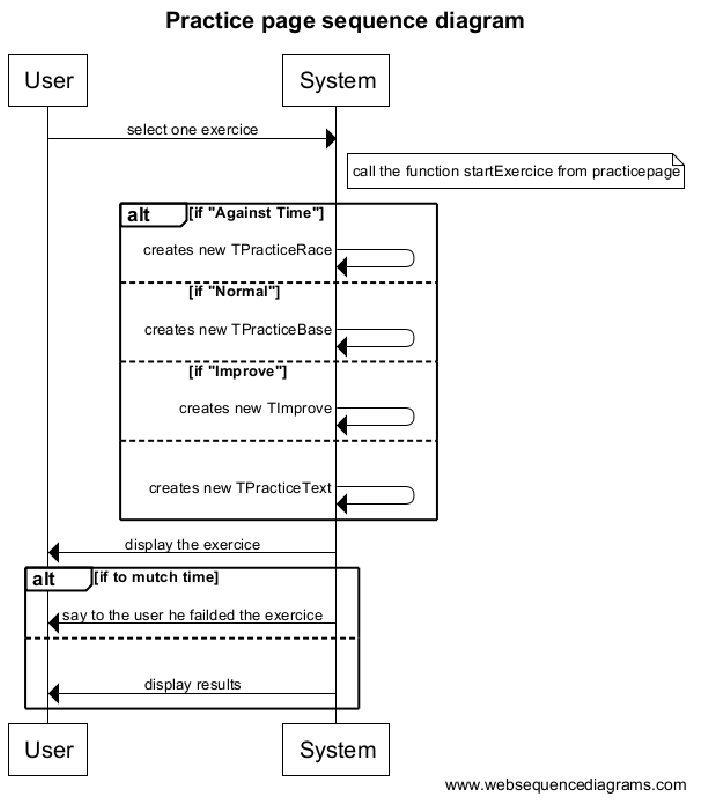
\includegraphics[width=12cm]{diagrams/Spracticepage.png}
    \caption{Sequence diagram for Practice page}
    \label{Spracticepage}
\end{figure}
\begin{figure}[H]
	\centering
    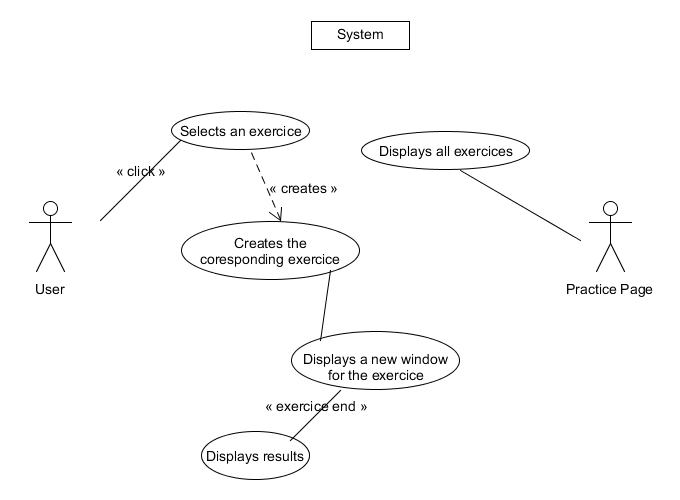
\includegraphics[width=12cm]{diagrams/UCpracticepage.png}
    \caption{User case diagram for Practice page}
    \label{UCpracticepage}
\end{figure}

Next figures respectively shows the relationship diagram (figure\ref{Rgamepage}), the sequence diagram (figure\ref{Sgamepage}) and the Use Case diagram (without details) (figure\ref{UCgamepage}) for the game page. Basically, the game page works like this:
\begin{itemize}
\item The user has already start the software and selected a user.
\item Actually there is just one button in the game page so when the user click on it(or on a future one), the system is starting the appropriate game in a new window.
\end{itemize}

\begin{figure}[h]
	\centering
    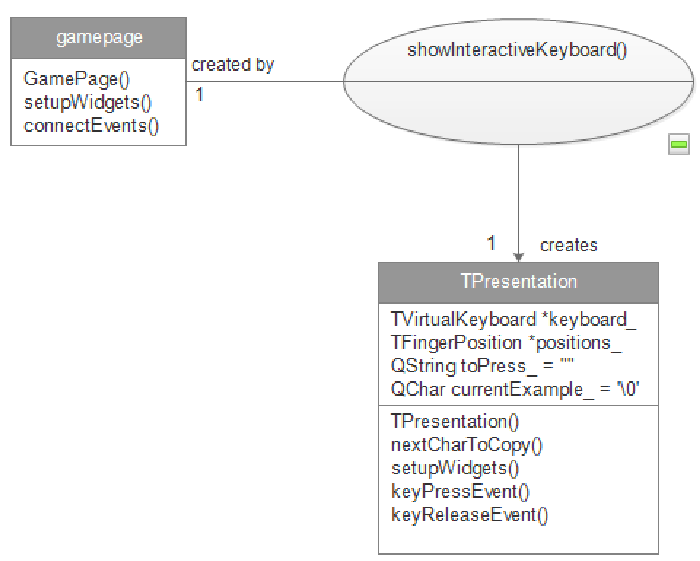
\includegraphics[width=12cm]{diagrams/Rgamepage.png}
    \caption{Relationship diagram for Game page}
    \label{Rgamepage}   
\end{figure}
\begin{figure}[h]
	\centering
    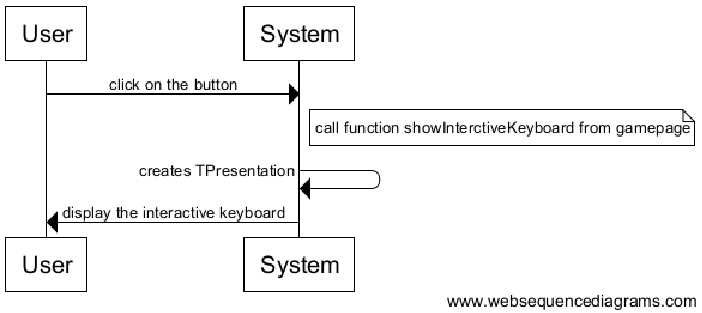
\includegraphics[width=12cm]{diagrams/Sgamepage.png}
    \caption{Sequence diagram for Game page}
    \label{Sgamepage}
\end{figure}
\begin{figure}[h]
	\centering
    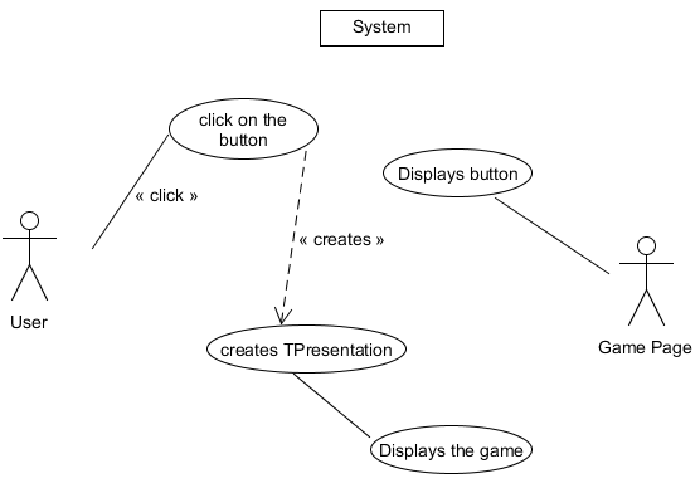
\includegraphics[width=12cm]{diagrams/UCgamepage.png}
    \caption{User case diagram for Game page}
    \label{UCgamepage}
\end{figure}

%------------------------------------
% Fin Partie Pierre
%------------------------------------



%Partie Azarias
%------------------------------------%
% Début Partie Azarias				%
%------------------------------------%
\part{System design}

\chapter{User interface design}
Because the project was created with Qt, and Qt adapt its interface depending on the OS it's running on, there is no 'global' user interface. However, the layout is always the same and so is the content. The following screenshots will show the user interface as it is on Linux, more precisely Ubuntu. Currently, QTypingTest is available on Ubuntu and windows.\\
When the user starts the software, he's directly directed on the homepage, figure \ref{homepage-logout} where he can either create a new profile or connect himself to his own existing profile. The buttons allowing to go through the differents part of the software are disabled as long as no one is connected. A list of the existing user is displayed and the user just has to click on his alias to be considered as connected(figure \ref{homepage-login}. He can then go through the differents part of the user interface. 
\begin{figure}[H]
  \centering
  \begin{minipage}[b]{0.45\textwidth}
    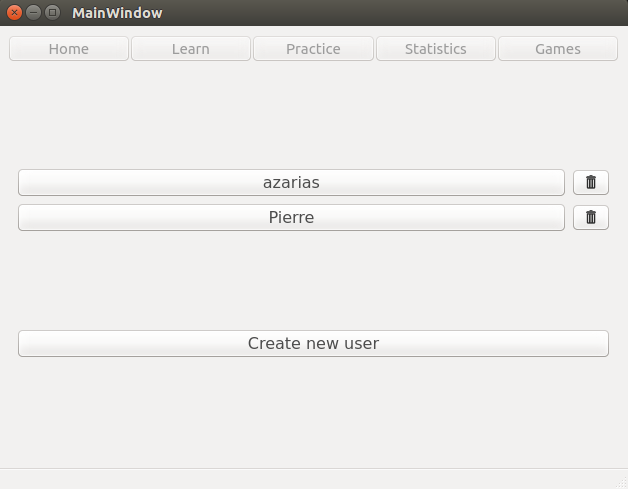
\includegraphics[width=\textwidth]{images/homepage_logout.png}
    \caption{Defaults homepage.}
    \label{homepage-logout}
  \end{minipage}
  \hfill
  \begin{minipage}[b]{0.45\textwidth}
    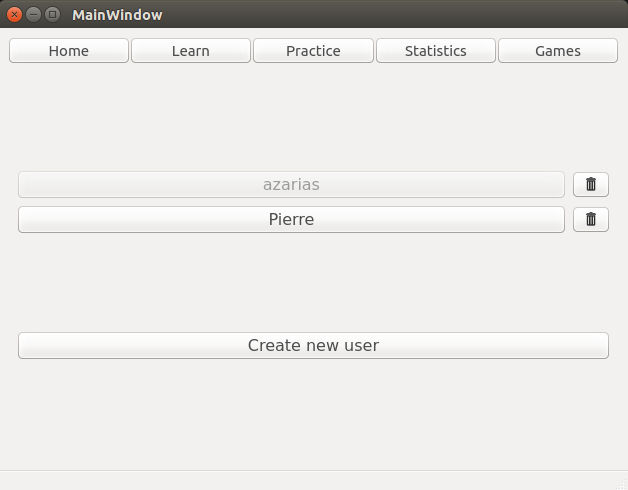
\includegraphics[width=\textwidth]{images/homepage_login.png}
    \caption{User connected.}
    \label{homepage-login}
  \end{minipage}
\end{figure}
A user can also delete his profile by clicking on the trash icon. \\
The purpose of the login system was not to be secured. Since this software is made for private use, and that it does not contain any sensible informations, the group decided to focus on the software itself and to do not spend to much time on the login system. \\
On the top of the window, there are five buttons.
\begin{itemize}
	\item Home. This button, when triggered, shows the homepage, but does not disconnect the user.
	\item Learn. This show the main part of the project. The page where the user has a list of the differents letters to learn in an certain order.
	\item Practice. On this page, the user can choose differents mode of practice.
	\item Statistics. Here, the user can see his statics.
	\item Games. Some simple games developed to learn the fun way to type.
\end{itemize}


\begin{figure}[H]
	\centering
	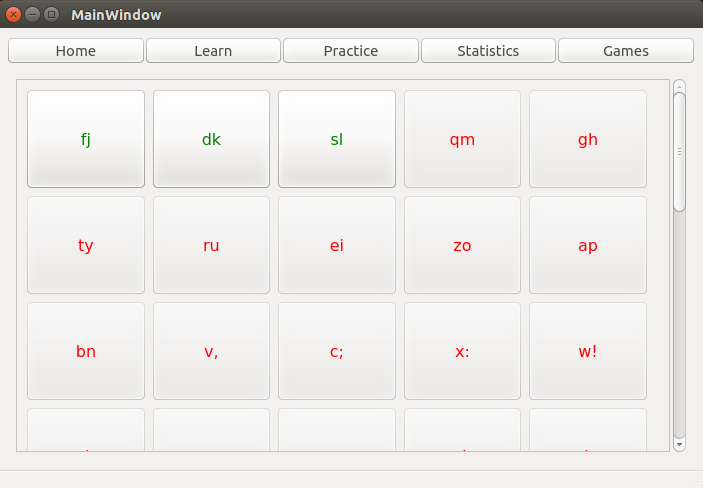
\includegraphics[width=0.7\textwidth]{images/page-learn.png}
	\caption{Learn page}
	\label{page-learn}
\end{figure}

The learn page (figure \ref{page-learn}) the user can see all the exercises to come. He must succeed to them one by one. And should realize a minimum score the be able to unlock the next exercise. When clicking on a button, a dialog is shown and the user can start a new exercise.

\begin{figure}[H]
	\centering
	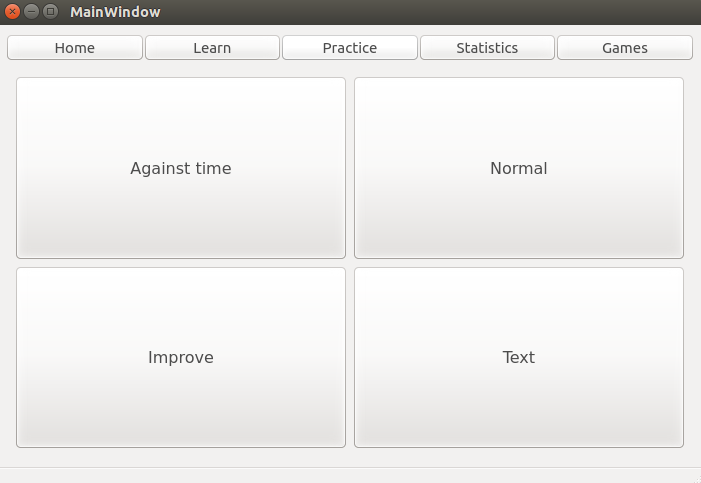
\includegraphics[width=0.7\textwidth]{images/page-practice.png}
	 \caption{Practice page}
	 \label{page-practice}
\end{figure}

The practice page  (figure \ref{page-practice}) has four buttons. One for each differents type of practice. The final 'form' of each practice is always the same : a dialog with text to type. What's changing is the content of the dialog.\\
The differents rules for each types of practice are 
\begin{description}[align=left]
	\item[Against time :] The user must type the most words in one minute. At the end of this time, his number of words per minute is shown.
	\item[Normal :] The user has two 'pages' of random words to type. Thanks to the powerful language system of Qt, the displayed words may change depending on the user's computer language. For the moment, only english and french is supporter.
	\item[Improve :] This practice will check what is the user's worst letters and create a special exercise containing these letters.
	\item[Text :] In this practice, the user will have to type an existing text. The chosen text are the 'classical' authors such as George Orwell. Once again thanks to Qt, the language of the text may vary depending on the user's computer language. The default language being english. 
\end{description}

\textit{The statistics page was not made yet}

\begin{figure}[H]
	\centering
	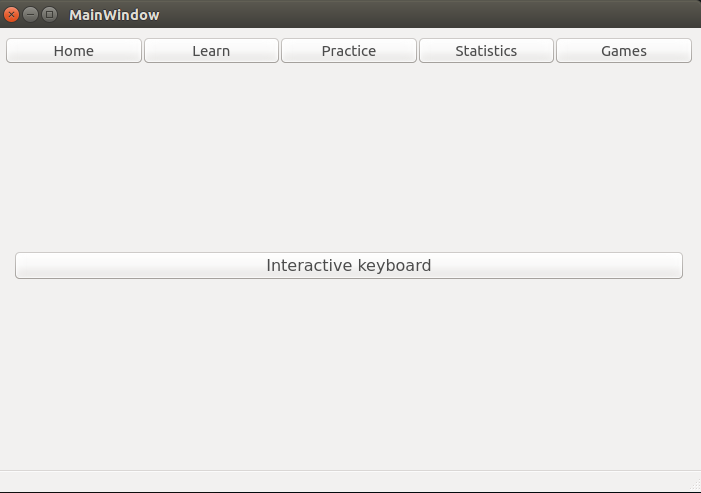
\includegraphics[width=0.7\textwidth]{images/page-games.png}
	 \caption{Game page}
	 \label{page-game}
\end{figure}

The game page contains a single button. This button launches a dialog where the user sees what letters is associated with what finger on the keyboard.

\subsection{The differents dialogs}
Here are the dialogs that can be opened with Qt :

\begin{figure}[H]
	\centering
	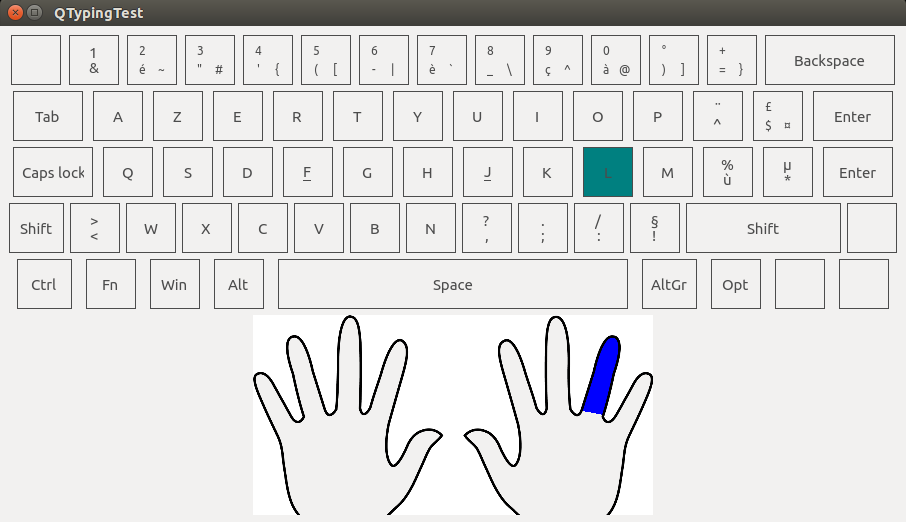
\includegraphics[width=0.7\textwidth]{images/dialog-before-learn.png}
	 \caption{Before the learning dialog}
	 \label{dialog-before-learn}
\end{figure}

Here is the dialog shown when the user starts an exercise to learn new letters.\\
This dialog highlights in a certain color the finger and associated with the letter on the keyboard. This invites the user to do the same. Thus use the indicated finger to type on the indicated letter. When he does this, the next letter and the next finger highlights. When those two steps are completed, the user can start the real exercise.\\
The pictures shows the configuration of an AZERTY keyboard, because the test are made on a french computer. But a configuration file is also made for QWERTY keyboard, and anyone who uses a non-french computer's configuration will automatically have the QWERTY configuration loaded.

\begin{figure}[H]
	\centering
	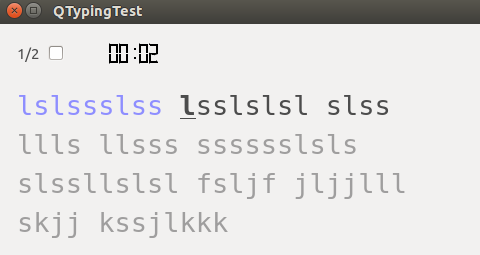
\includegraphics[width=0.7\textwidth]{images/dialog-learn.png}
	 \caption{The learning dialog}
	 \label{dialog-learn}
\end{figure}

The figure \ref{dialog-learn} shows the dialog to learn new letters. In this case, the letters are \textit{S} and \textit{L}.\\
There are two parts on the dialog : the toolbar and the center part.\\
The toolbar contains :
\begin{itemize}
	\item The page indicators that tells on what page is located the user and how many remains.
	\item The play/pause button as the check-box button. When it's toggled the game is paused and when it is not (the default) the game goes on.
	\item The timer. This tells the user how much time was spent since the start of the exercise.
\end{itemize}

The center part contains the user's exercise. It displays a text on two pages with four color codes :
\begin{itemize}
	\item Black : a normal black letter is a letter to be typed in the future
	\item Black underlined and bold : the current letter that the user has to type
	\item Blue : a letter already typed by the user and correctly typed
	\item Red  : a letter already typed by the user but incorrectly typed
\end{itemize}

The center part does not takes care of the words. It's only taking care of each letters.\\
The user can rewind back to retype the letters. This will also work from one line to another. However this is voluntary not possible
from one page to another.\\
This dialog will always look the same for the trainings and the exercise. The only difference lives in the content of the main part.\\
For the exercise dialog, the exercise is organized as so :
\begin{enumerate}
	\item For two lines, only the two letters that the user must learn.
	\item For two lines all the letters previously learned in a random order
	\item And the remain part is some random words with the letters previously learned. If no words can be made with the letters learned (especially true at the beginning) the second part will be repeated.
\end{enumerate}

\begin{figure}[H]
	\centering
	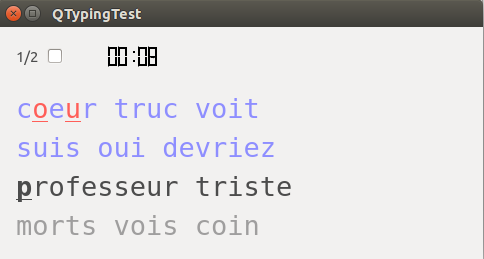
\includegraphics[width=0.7\textwidth]{images/dialog-practice.png}
	 \caption{The practice dialog}
	 \label{dialog-practice}
\end{figure}

This dialog is very similar to the learning dialog. The toolbar is exactly the same and works the same way.\\
The only difference is the content. This dialog contains only real words. In this case, it's only french words since there is a words file for french computers. There is also a file containing english words. And this file is the default one.\\
This type of exercise contains only words placed in a random order, on two pages.

\begin{figure}[H]
	\centering
	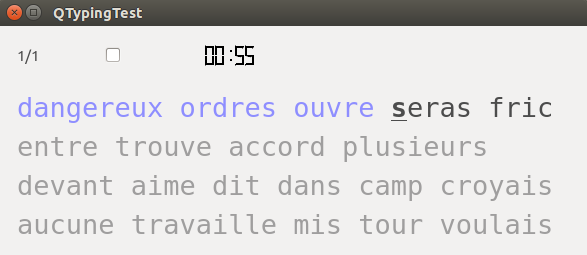
\includegraphics[width=0.7\textwidth]{images/dialog-race.png}
	 \caption{The race dialog}
	 \label{dialog-race}
\end{figure}

The race dialog is similar to the two previous one. However there is one difference in the toolbar. Instead of starting at 0, the timer starts at 1 minute, and decreases. This changes results in another change : the number of pages. Since the number of page depend on the speed of the user. It is 'unknown'. But instead of hiding this information, it will simply increase for each new page created.\\
For this exercise, only one page is generated and if the user succeed to finish the page, another one is generated and displayed. Thanks to the speed of C++ and the algorithms, the user does not see the difference. This system allows the exercise to generate (in theory) an infinite number of pages and therefore change the start time.
The content is the same as the practice dialog : it contains only words of french or english depending on the user's computer (in this case, french).\\

\begin{figure}[H]
	\centering
	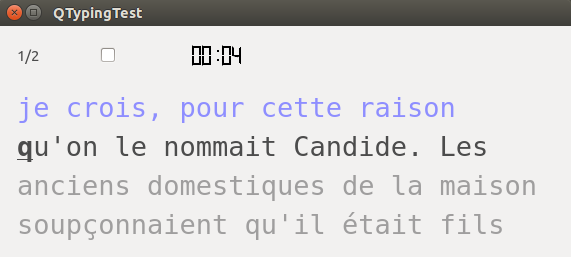
\includegraphics[width=0.7\textwidth]{images/dialog-text.png}
	 \caption{The text dialog}
	 \label{dialog-text}
\end{figure}

The text dialog is exactly the same as the practice dialog. The only difference is the content. Instead of containing only random words, it contains a real text. The text is either in french or english, depending on the user's computer configuration.

\begin{figure}[H]
	\centering
	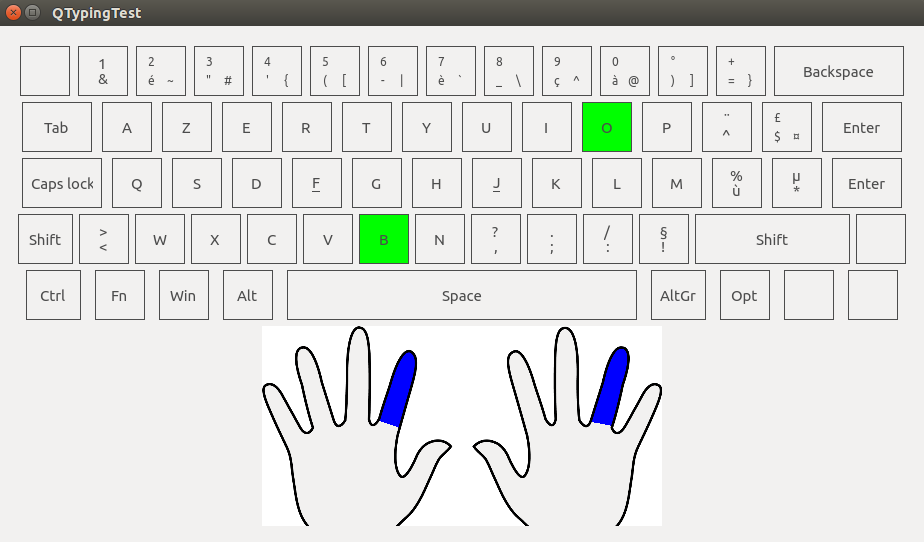
\includegraphics[width=0.7\textwidth]{images/dialog-game.png}
	 \caption{The game dialog}
	 \label{dialog-game}
\end{figure}

The game dialog is the same as the one shown before the learning exercise. But instead of showing the user what letter he has to type, it will simply let him free to type whatever letters he wants, and shows what finger is associated with this letter. \\




\section{Qt features}

Qt is a really powerful framework full of features. There are so many of them that is sometimes possible to miss one and redo all the work. That's what happened for the group many times during the development of the software.\\
Qt is first made to create user interfaces on great variety of OS. With the same source code, it is possible to have a interface for linux, windows and mac OS. But there are a lots of useful features to improve the life of the developer and some tools to improve the C++ language.\\
The most powerful feature by far of Qt is it's SIGNAL-SLOT system.

\begin{figure}[H]
	\centering
	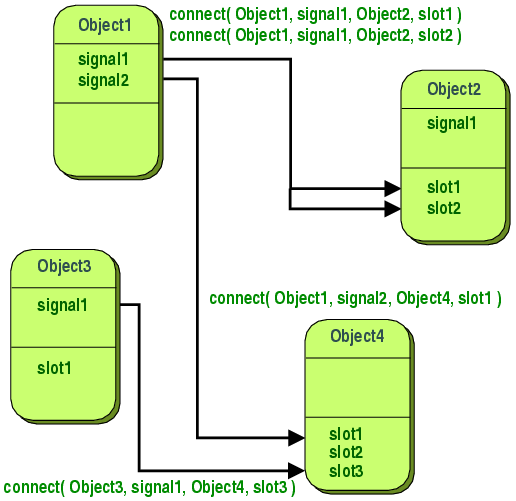
\includegraphics[width=0.7\textwidth]{images/abstract-connections.png}
	 \caption{The connection system in Qt}
	 \label{signal-slot-qt}
\end{figure}

The figure \ref{signal-slot-qt} shows how it works.
A signal can be emitted and a slot can be called whenever a signal is emitted. This is very useful to program interactive user interfaces.\\
It would be too long to enumerates all the features that Qt provides, and a lots of them where not used in the project. However, here is a list of features used for the project provided by Qt.

\begin{description}[align=left]
	\item[Language detection] : Qt can easily detect the user's computer language. This was first used to select the files for the exercises.
	\item[Resources files] : The group discovered later than Qt can actually automatically select the good file depending on the computer language. This is made thanks to a resource file (.qrc). This file is written in XML and tells Qt where to find the resource file, give them a language and give them an alias. Then, when needing a file in the code the alias of the file is given, and Qt will choose the good file depending on the computer's language.
	\item[DataStream] : It is possible with Qt to open and read or write in a file. This 	was first used to save the users in binary files. The files can also be opened in text mode to read and write UTF8-only characters. This was used to read the keyboard configuration files.
	\item[Qt Variant and metatypes] : as for the language detection, the group discovered later that Qt has a pre-made data-saving system. This provides a safer way to save the data on the computer. Instead of writing on a file in the folder of the project itself, Qt will choose a system folder depending on the OS of the computer to write down the data to save.
	\item[Json] : Qt supports the JSON format. It can parse any valid json file and be used later on in the code. This is what's actually used to save the keyboard configurations. 
	\item[XML] : As for the JSON, Qt also support XML. It can parse any XML file and return an object that can be manipulated easily. This features could have been used to save the texts.
	\item[QString] : Last be not least. Qt provides a really powerful class : the QString. This class is really easy to use, and full of functions.
\end{description}

\subsection{Documentation}
It is not a part of Qt itself, but without it, the development of the software would be impossible.\\
The documentation of Qt is available online, but also on QtCreator. It is really well-made. Easy to read comprehensive, completed with examples and consistent.\\
Moreover, when there is a problem with Qt and that the documentation cannot solve the problem, the community behind Qt is huge and really helpful.  

\chapter{Functional Design}
This project is relatively simple an contains two main parts :
\begin{description}
	\item[The learning] : where the user learn each letters of the keyboard one by one
	\item[The practising] : where the user can see the progress made by typing real words, and real texts
\end{description}
Since this software is quite simple, everyone with a computer can use it. This means the software is made for all ages. Anyone whether there are young, can use the software without a lot of explanation and learn, step by step how to correctly use his keyboard.\\
Also, thanks to Qt robustness and features, the software is viable and is unlikely to crash during its usage.

\section{Structure of the system}

\begin{itemize}
	\item The Data part. This part is where all the objects containing data are stored. e.g the users, his statistics ... 
	\item The User interface part. This part contains all the files necessary to create the user interface. All the classes in this parts inherits at least of QWidget (which is the base element for the GUI).
	\item The utils part. In this part, there are no classes, only namespaces. Theses class are here to facilitate the developer's life and provides useful functions to make the software work.  
\end{itemize}

Those three parts are separated in three different folders (namely "Data","QTypingpTest" and "Utils").\\

This separation was creating a pseudo-pattern of MVC. The model being the data, the View being the GUI and the Utils being the controller. However, for programming reasons, the main parts of the controller was situated in the view itself. Because thanks to the signal slot (figure \ref{signal-slot-qt}) system, the function used as controller could be in the GUI itself.



\section{Code walkthrough}
Begin with the beginning : the main.
\begin{lstlisting}
#include <QApplication>//The application
#include <QDebug>//The logger
#include <QDir>
#include <time.h>//Random number 
#include <QFile>
#include <QTranslator>//Computer's locale
#include <QLocale>
#include <QLibraryInfo>

#include "QTypingTest/thomepage.h"

void init(){
    srand(time(NULL)); //Random number generation

    qRegisterMetaTypeStreamOperators<TUser>("TUser"); //Metatype declaration

    //Set translator
    QString locale = QLocale::system().name().section('_',0,0);
    QTranslator translator;
    translator.load(QString("qt_") + locale,QLibraryInfo::location(QLibraryInfo::TranslationsPath));
    QApplication::installTranslator(&translator);
}


int main(int argc, char *argv[]) {
    QApplication a(argc, argv);//Start Qt

    init();   //Register the type to be able to create QVariant from them

    THomePage hp;

    //Set style
    QFile file(":/style.qss");
    if (file.exists()) {
        if (!file.open(QIODevice::ReadOnly | QIODevice::Text)) {
            qDebug() << "Could not open file, please check the permissions";
        } else {
            hp.setStyleSheet(QLatin1String(file.readAll()));
        }
        file.close();
    } else {
        qDebug() << "Could not load stylesheet";
    }


	//Show the main window
    hp.show();

	//enter qt's main loop
    return a.exec();
}
\end{lstlisting}

This code is very interesting since it shows a lot in a few lines of code. Here is step by step, what is happening :
\begin{description}
	\item[Creating the qt application object.] To run qt, an application must be created, otherwise, there is no main loop and no window to display
	\item[init.]  This function contains a series of initialisation :
	\begin{itemize}
		\item initiate the random number generation
		\item Register the TUser type to be able to read saves 
		\item install the translator by detecting the computer language.
	\end{itemize}
	\item[Set the style.] Qt support a CSS format. This style can be applied to the elements of the GUI. Since almost all basics CSS directives are supported, it's easy customize the GUI.
	\item[Show the main window.] The homepage was already created before. Now  it is time to display it since all the initialisation is done.
	\item[Enter the main loop.] To let the window opened an really launch the software once for all. The last line does this for us.
\end{description}

\begin{lstlisting}
void THomePage::connectEvents() {
    TUserManager::getInstance().readUsers();
    connect(ui.action_option,SIGNAL(triggered(bool)),this,SLOT(showOptionDialog()));
    connect(ui.action_aboutQt,SIGNAL(triggered(bool)),qApp,SLOT(aboutQt()));
    connect(&TUserManager::getInstance(),&TUserManager::usersSaved,this,[=](){
        ui.statusbar->showMessage("Users saved !",4000);
    });
    connect(&TUserManager::getInstance(),SIGNAL(userChanged(TUser*)),this,SLOT(updateUI(TUser*)) );

	//Associate 
    buttonsStacks_[ui.button_home] = ui.page_home;
    buttonsStacks_[ui.button_learn] = ui.page_learn;
    buttonsStacks_[ui.button_games] = ui.page_games;
    buttonsStacks_[ui.button_stats] = ui.page_stats;
    buttonsStacks_[ui.button_practice] = ui.page_practice;

    //Iterate over the buttons-page couple
    for (auto it = buttonsStacks_.begin(); it != buttonsStacks_.end(); ++it) {
        //If child is not nullptr create a simple layout with parent and add the child into it
        if (!TUserManager::getInstance().getCurrentUser()) {
            it.key()->setEnabled(false);
        }

        connect(it.key(), &QPushButton::clicked, [ = ](){
            ui.stack_main->setCurrentWidget(it.value());
        });
    }
    ui.stack_main->setCurrentWidget(ui.page_home);
}
\end{lstlisting}
This function is called in the constructor of the the main window. What is intersting to see here is the signal-slot system of Qt.
Here is the list of what this function does :
\begin{description}
	\item[Read the users.] Will load the QSettings saved from the previous session into the usermanager
	\item[Connect the toolbar actions.] The toolbar contains actions, these are connected to several function of the main window
	\item[Associate the buttons with the pages.] The main window contains differents buttons. Each one is changing the current page.
	\item[Show the homepage.]
\end{description}

The signal-slot is used in this function. This line : 
\begin{lstlisting}
connect(&TUserManager::getInstance(),SIGNAL(userChanged(TUser*)),this,SLOT(updateUI(TUser*)) );
\end{lstlisting}
is an example of a connection. It means : on the instance of Usermanager, when the signal 'userChanged' is emitted, qt will trigger the function 'updateUI' of the main window.\\
There are several ways to connect a signal to a slot. Another way used in the code above is the anonymous function. C++11 introduced the anonymous functions. It is possible to use it as so in qt :
\begin{lstlisting}
connect(it.key(), &QPushButton::clicked, [ = ](){// < start of anonymous function
	ui.stack_main->setCurrentWidget(it.value());
});//< end of anonymous function
\end{lstlisting}



\chapter{Data design}
All the data is stored in objects when the software is running. Which also mean it is stored in the RAM of the computer.
The 'problem', is that when the software is not running, the objects are cleared, and not kept in the RAM. The solution the group used to overcome this problem is to use Qt's saving system called QSettings. Fortunately all the data to save, is the user statistics.\\
This figure shows all the user's data :

\begin{figure}[H]
	\centering
	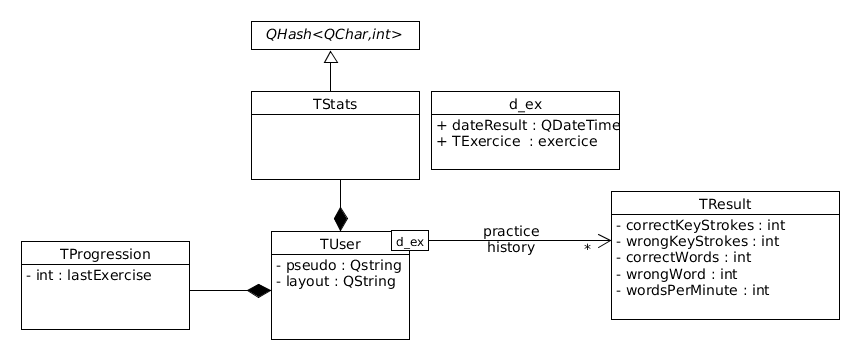
\includegraphics[width=0.7\textwidth]{images/diagram-data.png}
	 \caption{The user's data}
	 \label{diagram-data}
\end{figure}

All the objects represented contains two functions :
\begin{itemize}
	\item One to save the object itself (operator <<)
	\item One to create the object from a save (operator >>)
\end{itemize}

So every time a user was saved, the first function of every object was called, and at the start of the software, all the objects were loaded from the ROM to the RAM by calling the second function. The QSettings class to save the users was voluntary chosen. Since the model is not complex and a very few object are in relationship, the group chose to use QSettings. \\
However, Qt also supports the database operations and provide a support for sqlLite. As said above, there is also a support for XML and JSON. Those last two were not chosen two prevent easy cheating.


\part{System implementation}

\chapter{Building the software}
\section{First prototype}
The first prototype that the group presented to the first demo was giving an idea of the project. It was really fast to build and was containing only one window. On which the user could write down a text. It was a sort of 'proof of concept'. The purpose of this prototype was to demonstrate the main feature of the software and it was also a starting point for the group.\\
The first prototype was containing only two C++ classes. One for the whole window, and one for each row. Even if the prototype was working well, the interface was not very user-friendly and an offset could easily appear when the user was making too many mistakes.
Meaning that even if the prototype was working, a lot of work would be necessary to improve the user interface. \\
This prototype was also a sort of training for the group, it was the first window ever made with Qt. Because the group members didn't know anything about Qt, it was absolutely normal to have such a poor interface.

\section{Second prototype}
The second an actual prototype is a lot more evolved than the first prototype. There are more features, it's working better and it's more user-friendly. Of course, there is some improvements that remains possible.\\
However, the software is ready for production and can be used by anyone who wants to.\\
The second prototype started with a big improvement of the first prototype. The two lines : one for the text, and one for the text-field where the user can type were merged into a single one. So, as the user would type the text, the current character would be displayed in a certain color, the future characters would also be displayed as 'passed'. Therefore, the offset problem was solved. Thanks to the support of HTML in the label with Qt, the task was quite easy.\\
Now that the group had a functional and user-friendly base, they could start to work on the other parts of the project and use this base for differents features.\\
Here are the list of features that were developed on this base, by order of development :
\begin{enumerate}
	\item random-letters typing. Were the user has to type a random set of letters
	\item random-words typing. Were the user has to type real words
	\item text typing. Were the user has to type an existing text (written by great authors such as George Orwell)
	\item improvement. This exercise is using the statistics of the user to know what mistake is the more frequent
\end{enumerate}
All these differents exercise has its own class. But they also all inherit from the same base class to have access to the same resources such as a timer, a play/pause button, and a score a the end.\\
Then the group worked on different aspects of the main program, such as an interactive keyboard, the user's statistics and a homepage where a use can create its account, connect/disconnect.


\chapter{Current state of the software}
The current state of the software is complete. The software is available on \url{github.com} and can be downloaded for Linux or Windows. Anyone with a computer can download the software and start to learn how to type !
Even if the system is working well, the GUI is improvable. However, since the group is not design experts, they did as they could to create a usable software that does not hurt the eyes. And because the software is made up in C++, it's a bit harder than the web to stylize the interface. Even though Qt provides a CSS-like feature to change the style of every elements in a window.


\part{Testing}

\chapter{Unit testing}
Really early in the development of the software, it became obvious that some key features required unit testing.\\
Luckily Qt provides a way to easily and quickly create unit testing. All the tests of the projects are on the 'test' folder.\\
The tests for this projects were created for two main purpose :
\begin{enumerate}
	\item ensure that the feature are working as expected
	\item avoid compiling all the project for a single feature test
\end{enumerate}
Some test requires the GUI some does not. The hard part of the test was not to create them, it was to make the software testable. For example, a lots of features held on randomness. And it is not possible (or silly) to test randomness. This means, the less randomness, the more testable. Or pseudo-random features were testable.

\chapter{GUI testing}
GUI testing

\part{Usability - Users tasks}
Usability - Users tasks

\chapter{What can the user do}
What can the user do


\chapter{Efficiency and response times}
Efficiency and response times

\chapter{Overall aesthetic}
Overall aesthetic

\part{Conclusion and further work}
Conclusion and further work

\chapter{Project result}
Project result

\chapter{Possible improvements}
Possible improvements

\chapter{Further work}
Further work
%------------------------------------%
% Fin Partie Azarias					%
%------------------------------------%


%------------------------------------%
% Début Partie commnune				%
%------------------------------------%
\part{Personal reflections on project experiences}
Personal reflections on project experiences

\chapter{Pierre Thubé}
In view of the final software, I think we can say that principal goals has been reach. This project bring me knowledge in C++ and about the framework Qt. However, it also show me some of my weaknesses for example about how fast I am working. I would have like to be able to do more to learn more but with all works we had during the year and the gap of level between Azarias and me about C++ or way to learn new things, I had the feeling sometimes to be outworn by all the amount of work. However, I am still satisfied to have discovered Qt framework and this project confirm me that I prefer computer language like C++ or Java (object oriented language).\\
I also discovered how was working git and even if we was just using the bases, it will be helpful for the next time I will need it. 

\chapter{Azarias Boutin}
I am quite satisfied with the software developed. When the group started the project, I was knowing nothing about Qt and wanted to learn as much as possible about this amazing framework. I knew the basics of C++ and felt this would be enough to build a good software. I also knew the basics of GUI thanks to the lessons with java swing. I really felt that this project bring me a lot of knowledge. During the implementation of the software, the several improvement steps proved this point.\\
However, I also feel like the project was not progressing fast enough. Maybe because of a lack of communication but also because of lack of knowledge from the other group member. Furthermore, since the group was only composed of two members, I felt like I was carried all the project from the beginning to the end.\\
Overall I am satisfied with the result and the software developed. It was a rich experience, and I learned a lot about Qt. I also learned a lot about git and version management system.


\end{document}